\documentclass[11pt,a4paper,twoside]{thesis}

\usepackage{graphicx}
\usepackage[utf8]{inputenc}
\usepackage[spanish]{babel}
\usepackage[left=3cm,right=3cm,bottom=3.5cm,top=3.5cm]{geometry}
\usepackage{titlesec}
\usepackage{listings}
\usepackage{xcolor}
\usepackage{hyperref}
\usepackage{amsmath}
\usepackage{amssymb}
\usepackage[utf8]{inputenc}
\usepackage{enumitem}
\usepackage{booktabs}

\begin{document}

%%%% CARATULA

\def\autor{Adrian Norberto Marino}
\def\tituloTesis{Sistemas de Recomendación Colaborativos}
\def\runtitulo{Resumen}
\def\runtitle{Sistemas de Recomendación Colaborativos}

%\def\director{Obi-Wan Kenobi}
%\def\codirector{Master Yoda}

\def\lugar{Buenos Aires, 2022}

% -----------------------------------------------------------------------------
% Caratula,  Resumen, agradecimientos y dedicatoria.
% -----------------------------------------------------------------------------
\newcommand{\HRule}{\rule{\linewidth}{0.2mm}}
%
\thispagestyle{empty}

\begin{center}\leavevmode

\vspace{-2cm}

\begin{tabular}{l}

\includegraphics[width=3.6cm]{./images/logouba.png}
\end{tabular}


{\large \sc Universidad de Buenos Aires\\Facultad de Ciencias Exactas y Naturales \\ Facultad de Ingeniería}

\vspace{6.0cm}

\vspace{3.0cm}
%{
%\Large \color{red}
%\begin{tabular}{|p{2cm}cp{2cm}|}
%\hline
%& Pre-Final Version: \today &\\
%\hline
%\end{tabular}
%}
%\vspace{2.5cm}

\begin{huge}
\textbf{\tituloTesis}
\end{huge}

\vspace{2cm}

{\large Trabajo Final de la \textit{Especialización en Explotación de Datos y Descubrimiento del Conocimiento}}
\vspace{2cm}

{\large \href{https://github.com/adrianmarino/thesis-paper}{Github Project}}

\vspace{2cm}

{\Large \autor}

\end{center}

\vfill

{\large

%{Director: \director}

\vspace{.2cm}

%{Codirector: \codirector}

\vspace{.2cm}

\lugar
}

\newpage\thispagestyle{empty}

%
\frontmatter
\pagestyle{empty}
%\begin{center}
%\large \bf \runtitulo
%\end{center}
%\vspace{1cm}
\chapter*{\runtitulo}

\noindent Este trabajo cubre la comparación de sistemas de recomendación basados
en filtros colaborativos. Es una explicación exhaustiva del funcionamiento e
implementación de la batería de modelos de recomendación colaborativos mas utilizados
como son: \textit{GMF}, \textit{Biased-GMF}, \textit{KNN Item Based},
\textit{KNN User Based}, \textit{DeepFM} y \textit{NN-FM}. Se pretende comparar
todos los modelos, utilizando métricas especializadas como el promedio
de la precisión (\textit{AP@K}) y la media del promedio de la
precisión (\textit{mAP@k}), y otras menos especializada como la raíz
del error cuadrático medio \textit{RMSE}. Todos los modelos se entrenaron
utilizando el mismo \textit{dataset}, construido a partir de los
\textit{datasets} \textit{TMDB} y \textit{Movie Lens}. A grande rasgos,
se ha encontrado que no existe una diferencia sustancial en precisión
para los modelos propuestos. Por otro lado, se ha encontrado que modelo
basados en \textit{Deep Learning} obtiene resultados ligeramente superiores
a modelos mas clásicos, como la familia de modelos \textit{KNN}.

\bigskip

\noindent\textbf{Palabras claves:} Sistemas de Recomendación,
Basados en Filtro Colaborativos, Basados en Contenido,
Modelos Híbridos, \textit{GMF}, \textit{KNN}, \textit{NN-FM},
\textit{DeepFM}, \textit{mAP@k}.
%
%\cleardoublepage
%\chapter*{Agradecimientos}

\noindent  % OPCIONAL: comentar si no se quiere
%
\cleardoublepage
\chapter*{Agradecimientos}

\hfill \textit{Principalmente a mis padres, siempre fueron un gran apoyo en mi carrera, alentándome incansablemente para seguir adelante en todo momento. Gran parte de mi disciplina de constante persistencia se la debo a ellos. En segundo lugar a mis profesores de la especialización y maestría, por entregarnos su conocimiento dia a dia, siempre enfocados en que comprendamos todos los temas expuesto de la mejor forma posible. A mis compañeros de la especialización, siempre fueron un gran grupo de apoyo, un grupo en el que nos ayudamos uno al otro para comprender los temas expuestos.}
  % OPCIONAL: comentar si no se quiere
% -----------------------------------------------------------------------------
%
%
%
%\cleardoublepage
\tableofcontents
%
%
\mainmatter
\pagestyle{headings}
%
%
%
%
% -----------------------------------------------------------------------------
% Contenido de la tesis
% -----------------------------------------------------------------------------

\setitemize{itemsep=0.5pt}

\chapter{Introducción}

Los sistemas de recomendación tienen como objetivo principal proporcionar a los
usuarios productos, promociones y contenidos relevantes a sus preferencias o
necesidades. Estos sistemas permiten a los usuarios encontrar de manera más
fácil y eficiente lo que están buscando. Formalizando esta definición, podemos
decir que los sistemas de recomendación buscan ayudar a un usuario o grupo de
usuarios a descubrir ítems que se ajusten a sus preferencias, dado un conjunto
de ítems que puede ser extenso o en un amplio espacio de búsqueda.

Este objetivo puede variar dependiendo de cada negocio: Si consideramos un
\textit{e-commerce} de \textit{delivery} gastronómico, su propósito sería
ofrecer a los clientes platos relevantes a un precio asequible y con un tiempo
de entrega aceptable.

Si hablamos de un \textit{e-commerce} de productos, su objetivo consiste en
proporcionar a los usuarios aquellos productos que satisfacen sus necesidades,
a un precio que estén dispuestos a pagar. Además, se busca garantizar una
experiencia satisfactoria con los vendedores.

En el negocio de visualización de contenido (audio, video, texto, etc..), el
objetivo es acercar a sus usuarios contenido a fin a sus preferencias para
mejorar su experiencia en la plataforma.

El objetivo principal en todos los casos es mejorar la conversión. En el campo
del \textit{marketing}, se define la conversión como las acciones realizadas
por los usuarios que están alineadas con los objetivos de la empresa. Por
ejemplo, aumentar el volumen de compras en un \textit{e-commerce} de productos,
incrementar la cantidad de entregas mensuales en un \textit{e-commerce} de
\textit{delivery} gastronómico, aumentar las impresiones de publicidad en
aplicaciones de visualización de contenido, prolongar el tiempo de permanencia
en plataformas de \textit{streaming} de audio o video, entre otros. Existen
numerosos ejemplos en los que el objetivo común es mejorar la conversión y el
compromiso del usuario con la marca, es decir, el \textit{engagement}.

Desde un enfoque técnico, los sistemas de recomendación se utilizan para
predecir el grado de preferencia de un usuario con un artículo específico. Esto
se logra aplicando algoritmos de optimización que minimizan la diferencia entre
el grado de preferencia esperado y el grado de preferencia real del usuario.
También existen otros enfoques que utilizan medidas de distancia para
determinar este grado de preferencia. En secciones posteriores, exploraremos
estos conceptos con mayor detalle.

\clearpage
\section{Tipos de sistemas de recomendación}

A continuación, en la figura~\ref{fig:clasification}, se pueden observar las
diferentes categorías y sub-categorías de los sistemas de recomendación:

\begin{figure}[!htb]
	\centering
	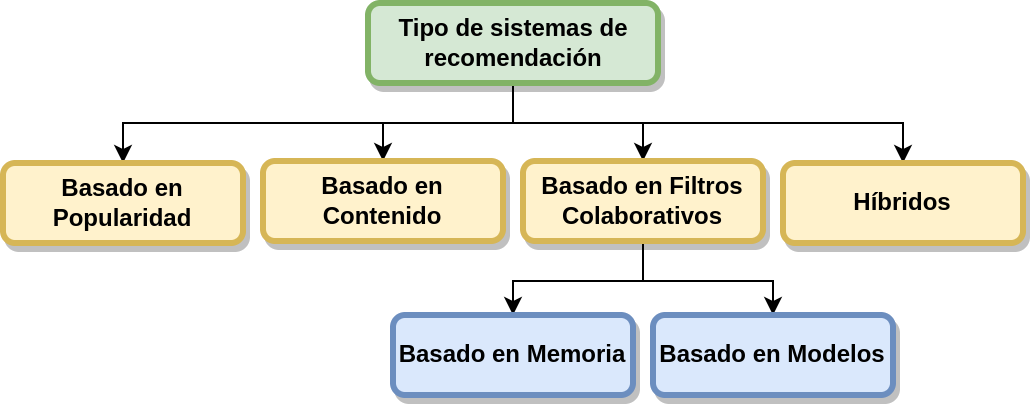
\includegraphics[width=12cm]{./images/clasificacion-sis-rec.png}
	\caption{Clasificación de tipos de sistemas de recomendaciones.}
	\label{fig:clasification}
\end{figure}

\subsection{Basados en Popularidad}

Este tipo de sistema de recomendación utiliza alguna característica de
popularidad de los ítems en cuestión. Algunos ejemplos de estas características
podría ser la cantidad de vistas, la cantidad de compras o la cantidad de
comentarios positivos, o una combinación de ellas. Luego, estos sistemas buscan
los K elementos más populares. Si bien este tipo de enfoque proporciona buenos
resultados para nuevos usuarios, sus recomendaciones no tienen en cuenta las
preferencias individuales de cada usuario, ya que se basan en estadísticas
comunes a todos los usuarios. Por esta razón, a menudo no se consideran
sistemas de recomendación en sentido estricto. No obstante, siguen siendo
ampliamente utilizados debido a su capacidad para generar una alta tasa de
conversión, a pesar de la falta de personalización.

\subsection{Basados en Contenido}

Este tipo de sistema de recomendación necesita un trabajo previo de ingeniería
de \textit{features} sobre los ítems. Se busca definir cuales son los
\textit{features} mas significativos para la tarea en cuestión, y cual es el
grado de adecuación de cada ítems a los \textit{features} seleccionados. Por
otro lado, es necesario registrar las interacciones de los usuarios. Dadas
estas interacciones, se puede definir el grado de preferencia de los usuarios a
cada \textit{feature} definido para los ítems. Con esta información, es posible
encontrar tanto ítems como usuarios similares y realizar recomendaciones del
tipo:

\begin{itemize}
	\item Dado el \textit{Usuario A}, el cual tiene preferencia por el \textit{Ítem X},
	      también podría tener preferencia por el \textit{Ítem Y}, por ser muy cercano o
	      similar al \textit{Ítem X}.
	\item Dos \textit{Usuarios A y B} cercanos o similares, tendrán preferencias
	      similares. De esta forma es posible recomendar ítem consumidos por el
	      \textit{Usuario A} al \textit{Usuario B} y vise versa.
\end{itemize}

La principal desventaja de este enfoque, es la necesidad de realizar ingeniería
de \textit{features} para encontrar los \textit{features} que produzcan
recomendaciones relevantes al usuario. El modelo no encuentra estos
\textit{features} automáticamente, sino que deben ser definidos de antemano
manualmente. Se puede apreciar que esto introduce un sesgo al momento de
seleccionar los \textit{features} o construirlos en base a datos referentes a
los ítems. Como ventaja, si se encuentran los \textit{features} correctos se
pueden lograr muy buenos resultados.

\subsection{Basados en Filtrado Colaborativos}

Estos modelos, a diferencia de los modelos basados en contenido, no requirieren
ingeniería de \textit{features}, lo que hace muy simple su implementación, ya
que únicamente es necesario registrar las interacciones de los usuarios para
con los ítems. Luego, el propio modelo encuentra automáticamente los
\textit{features} mas relevantes dependiendo de la cantidad de columnas que se
especifiquen (Dimensiones de un vector \textit{Embedding}). Ejemplos de
interacciones podrían ser:

\begin{itemize}
	\item El \textit{Usuario A} visualizo el \textit{Ítem X} el dia 2 de marzo de 2022.
	\item El \textit{Usuario A} compro el \textit{Ítem X} el dia 10 de marzo de 2022.
	\item El \textit{Usuario A} califico al \textit{Ítem X} con 5 puntos el dia 25 de
	      marzo de 2022.
\end{itemize}

Ambos tipo de modelos, basados en contenido y filtros colaborativos,
personalizan sus recomendaciones. Es decir, ajustan las recomendaciones a las
preferencias de cada usuario particular. Además, ambos permiten encontrar
usuarios e ítems similares y recomendar ítems entre usuarios similares.

Por otro lado, los modelos basados en filtros colaborativos, descubren un
espacio latente de soluciones sin necesidad de recolectar datos y definir
\textit{features} en forma manual, a diferencia de los modelos basados en
contenido. La selección o construcción manual de \textit{features} puede llevar
a una solución sesgada, ya que no esta basada en datos sino en el juicio
experto del científico de datos. Esto puede llevar a una selección subjetiva de
los \textit{features} que se aleje de la realidad, introduciendo un sesgo en la
predicción.

No todo son rosas con estos modelos, dado que sufren un problema llamado
\textit{Cold start} o arranque en frio. Los usuarios nuevos son aquellos que
aun no han realizado ninguna interacción con el sistema. Estos modelos no
podrán realizar recomendaciones a estos usuarios, dado que requieren un mínimo
de interacciones para comenzar a ofrecer recomendaciones con cierta precisión.

Además, existen otros problemas referidos al cambiar la cantidad de
interacciones de los usuarios. Si pensamos en una solución donde alimentamos al
modelo con una ventana de interacciones para los últimos N meses, tendremos las
siguiente situaciones:

\begin{itemize}
	\item Usuarios nuevos: Los usuarios nuevos no tendrán interacciones. Por lo tanto,
	      este modelo no podrá realizar ninguna recomendación. En general, se establece
	      un mínimo de interacciones para que el modelo pueda realizar recomendaciones de
	      forma acertada.
	\item Usuarios con pocas interacciones: Por otro lado, tenemos a los usuarios que
	      tienen una baja taza de interacciones con el sistema o aplicación. Por ejemplo,
	      en un \textit{e-commerce} de venta de productos, hay usuarios que compran con
	      mucha frecuencia y otros muy de vez en cuando. Estos últimos, en general
	      tendrán una baja taza de interacción pudiendo caer por debajo del umbral mínimo
	      que requiere el modelo. De esta forma, tendremos usuarios que quedarán fuera
	      del modelo actual.
	\item Usuarios con muchas interacciones: En este caso, el usuario tiene una gran
	      cantidad de interacciones con ítems. Para estos usuarios, el modelo podrá
	      ofrecer recomendaciones relevantes, ya que cuanto mas interacciones se tenga,
	      el modelo se ajusta con mas facilidad a sus preferencias. Por otro lado, esto
	      puede ser una gran desventaja, ya que se produce un efecto de túnel. Es decir,
	      el usuario obtiene recomendaciones muy ajustadas a sus preferencias, perdiendo
	      la capacidad de descubrir nuevos ítems que podrían ser relevantes. Por esta
	      cuestión se suelen mezclar tanto recomendaciones personalizadas como
	      no-personalizadas, para favorecer el descubrimiento de nuevos ítems.

\end{itemize}

\clearpage
\subsection{Modelos Híbridos}

Son aquellos modelos que combinan mas de una técnica de recomendación, también
llamados ensambles de modelos. Comúnmente están compuestos por modelos de
recomendación por popularidad, basados en contenido y filtros colaborativos. De
esta forma, cuando los usuarios caen por debajo del umbral de interacciones
necesarias por el modelo de filtro colaborativos, se utiliza un modelos basado
en contenido, popularidad, o algún otro modelo que no requiere de interacciones
del usuario para realizar sus recomendaciones.

\subsection{Categorías dentro de los modelos basados en filtros colaborativos}

Dentro de los sistemas de recomendación basados en filtros colaborativos,
tenemos dos sub-clasificaciones referidas a la forma en la que se realizan las
predicciones.

\subsubsection{Basados en Memoria}

Este tipo de modelos, como su nombre lo indica, mantiene sus datos en memoria.
Se recorren todos los datos (\textit{full scan}) cada vez que se necesita
realizar un inferencia o predicción (fijando un número de vecinos a comparar).
Un ejemplo de estos modelos es el algoritmo de k vecinos cercanos
(\textit{KNN}), el cual mantiene una matriz rala de distancias en memoria, la
cual se recorre completamente para comparar las distancias entre filas o
columnas, usando alguna medida de distancia como puede ser la \textit{distancia
	coseno}, \textit{coseno ajustada}, \textit{manhattan}, etc.. Para mitigar el
problema de búsqueda exhaustiva (\textit{full scan}), se puede utilizar una
memoria \textit{cache} y asi realizar estas búsquedas una única vez. Otro
problema es su limitación al tamaño máximo de la memoria con la que se cuenta,
es decir, que el tamaño de la matriz depende de la memoria máxima disponible.
Esto puede mitigarse utilizando implementaciones de matrices rala, las cuales
comprimen los datos en memoria guardando unicamente las celdas que tienen
datos. Además, es posible utilizar un memoria \textit{cache} que mantenga en
memoria las búsqueda mas frecuentes y baje a almacenamiento secundario las
menos frecuentes. Todos estos problemas de \textit{performance} y uso de
recursos se deben a que \textit{KNN} no reduce la dimensionalidad de los datos,
como si lo hacen varias implementaciones basadas en \textit{embeddings},
\textit{auto-encoder}, redes neuronales etc.., donde lo que se busca una
representación mas compacta de los ítems y usuarios sin perder información. Mas
allá de estos problemas, los resultados obtenidos por estos modelos no están
muy alejados de aquellos que se encuentran en el estado del arte. Puede
recomendarse su uso cuando tenemos un dominio reducido, dada su simplicidad.

\subsubsection{Basados en Modelos}

Algunos ejemplos de estos modelos son los clasificadores bayesianos, redes
neuronales, algoritmos genéticos, sistemas difusos y la técnica de
descomposición matricial (\textit{SVD}). Estos modelos en general buscan
directa o indirectamente reducir la dimensionalidad de los datos. De esta
forma, es posible utilizarlos en dominios con una gran cantidad de datos.

\clearpage
\section{Descripción del problema y motivación}

Con este trabajo se busca contestar las siguientes preguntas:

\subsection{¿Los modelos basado en filtro colaborativos que utilizan técnicos de \textit{Deep Learning}, obtienen mejores resultados que aquellas que no las utilizan?}

La idea detrás de esta pregunta es realizar \textit{benchmarks} sobre distintos
modelos del estado de arte basados en \textit{Deep Learning} o no, utilizando
el mismo set de datos y las mismas métricas. De esta forma, se busca comprender
cual es la diferencia en \textit{performance} entre los modelos seleccionados.
Por otro lado, se busca comprender cuando es mas adecuado utilizar cada
enfoque. Como ya se comentó en el apartado de introducción, hay modelos que
están mas limitados que otros según el número de recursos de \textit{hardware}
o interacciones con los que se cuenta.

\subsection{¿Cuáles son las ventajas y desventajas de cada enfoque a la hora de aplicar estas técnicas?}

Esta pregunta se refiere a comprender cuando es conveniente aplicar una técnica
u otra teniendo en cuenta las ventajas y desventajas de cada enfoque y modelo.

\subsection{¿Cómo se puede solucionar el problema de \textit{Cold start} que sufre el enfoque de recomendación basado en filtros colaborativos?} (Tesis)

Como ya se comentó en la introducción, los modelos de filtro colaborativos
necesitan un número mínimo de interacciones usuario-ítem para poder operar y
producir recomendaciones aceptables. La propuesta es explorar enfoques que
permiten lidiar con este problema. Uno de los enfoques más comunes es utilizar
ensambles de modelos basados en filtros colaborativos con otros modelo basados
en contenidos o popularidad. Estos ensambles puede diferir en sus técnicas
dependiendo del dominio de los datos.

\section{Objetivos}

Como primer objetivo, se pretender comprender cuales son los fundamentos
teóricos sobre los que se apoya cada técnica aplicada y bajo que escenarios
puede ser conveniente aplicarlas. Por otro lado, se intenta determinar cual es
la diferencia en \textit{performance} de cada técnica aplicada sobre el mismo
set de datos, midiendo su \textit{performance} utilizando las mismas métricas.
¿Obtenemos diferencias significativas?

Como segundo objetivo (Tesis), se busca proponer nuevas técnicas y/o explorar
técnicas existentes que permite lidiar o solucionar el problema de \textit{Cold
	start} que sufren los sistemas de recomendación basados en filtros
colaborativos. Ademas, se compararan esta técnicas mediante un
\textit{benchmark} propuesto, para compara como se comporta cada modelos ante
usuarios con escasas o ninguna interacción en el set de datos propuesto.

\chapter{Materiales y Métodos}

\section{Datos}

Para realizar este trabajo se selecciono el dominio del cine, ya que existen
conjuntos de datos bien definidos y actualizados. Estos \textit{datasets} en
general están pensados para probar modelos de recomendación. Por otro lado, es
el dominio clásico en \textit{papers} y literatura de sistemas de recomendación
en general.

Dada la propuesta de este trabajo, es necesario contar con datos de
interacciones de usuarios con ítems (Películas en este caso). Además, dado que
se busca solucionar el problema de \textit{Cold start} para el enfoque de
filtros colaborativos, se necesitará contar con otro enfoque de recomendación,
el cual posiblemente pueda ser basado en contenido. Por esta cuestión,
necesitamos contar con \textit{features} completos y consistentes para los
ítems (Películas).

Dadas estas necesidades, se decidió utilizar los \textit{datasets} expuestos a
continuación.

\subsection{\textit{MovieLens 25M Dataset}}

Este \textit{dataset}~\cite{movielens} prácticamente no tiene \textit{features}
para los ítems (Películas), pero si tiene la calificaciones realizadas por los
usuarios. También cuenta con un conjunto de \textit{tags} o palabras clave
cargadas por los usuarios para cada ítem (Película). Otro punto importante, es
que todos los usuarios tienen al menos $20$ interacciones, lo cual asegura no
tener problemas de baja \textit{performance} por falta de estas. De esta forma,
este \textit{dataset} sera muy util para entrenar modelos de recomendación
basados en filtros colaborativos. Además, cuenta con columnas extras como
\textit{tags}, que serán útiles a la hora de entrenar modelos basados en
contenido.

Por último, este \textit{dataset} contiene $25$ millones calificaciones, $1$
millón de \textit{tags} y $62.423$ películas. Estos datos fueron registrados
por $162.541$ usuarios entre el $9$ de enero de $1995$ y el $21$ de noviembre
de $2019$. A continuación en la tabla~\ref{table:movieLensColumns}, se
especifican las columnas del \textit{dataset}:

\begin{table}[!htb]
	\centering
	\footnotesize
	\begin{tabular}{l | p{0.8\linewidth}}
		\hline
		Columna            & Descripción                                                                                                                                                                                 \\
		\hline
		\textit{userId}    & Identificador univoco de un usuario.                                                                                                                                                        \\
		\textit{movieId}   & Identificador univoco de una película.                                                                                                                                                      \\
		\textit{timestamp} & Fecha en la cual el usuario calificó el ítem(\textit{movieId}). Es un string con formato año-mes. Existen valores entre 1997-09 y 2019-11 inclusive.                                        \\
		\textit{rating}    & Calificación del usuario. Es un valor discreto numérico: \textit{0.5}, \textit{1}, \textit{1.5}, \textit{2}, \textit{2.5}, \textit{3}, \textit{3.5}, \textit{4}, \textit{4.5} y \textit{5}. \\
		\textit{tags}      & Lista de palabras definidas por cada usuario, para una película. Dicho de otra forma escisten N \textit{tags} por cada par usuario-película.                                                \\
		\hline
	\end{tabular}
	\caption{
		Columnas del \textit{dataset} \textit{Movie Lens}, relevantes para este trabajo.
	}
	\label{table:movieLensColumns}
\end{table}

\clearpage

\subsection{\textit{TMDB Movie Dataset}}

Este \textit{dataset}~\cite{tmdb} no tiene calificaciones personalizadas para
los ítems como sucede con el \textit{dataset MovieLens} anterior, pero si tiene
varios \textit{features} referentes a películas. Estos \textit{features} pueden
ser muy útiles para modelos basados en contenido e inclusive modelos híbridos,
los cuales se busca explorar en el trabajo de tesis. Contiene datos de $5.000$
películas y sus columnas se especifican en la tabla~\ref{table:tmdbColumns} a
continuación:

\begin{table}[!htb]
	\centering
	\footnotesize
	\begin{tabular}{l | p{0.6\linewidth}}
		\hline
		Columna                                   & Descripción                                                                           \\
		\hline
		\textit{imdb\_id}                         & Identificador univoco de una película en la base de datos de \textit{IMDB}.           \\
		\textit{title y original\_title}          & Título y título original.                                                             \\
		\textit{release\_date}                    & Fecha de estreno.                                                                     \\
		\textit{status}                           & Define si la película fue estrenada o esta en desarrollo.                             \\
		\textit{overview}                         & Sinopsis de la película.                                                              \\
		\textit{poster\_path}                     & URL de imagen de portada de la película.                                              \\
		\textit{languages}                        & Lenguaje original y doblaje.                                                          \\
		\textit{genres}                           & Géneros.                                                                              \\
		\textit{adult}                            & ¿Solo es apta para adultos?                                                           \\
		\textit{popularity}                       & Índice de popularidad.                                                                \\
		\textit{vote\_count}                      & Cantidad de votos.                                                                    \\
		\textit{vote\_average}                    & Promedio de votos.                                                                    \\
		\textit{keywords/tagline} y \textit{tags} & \textit{tags} o palabras clase ingresadas por los usuarios para definir una película. \\
		\textit{budget}                           & Presupuesto destinado a la realización de la película.                                \\
		\textit{revenue}                          & Retorno de inversión o ganancias.                                                     \\
		\textit{production\_companies}            & Compañías que produjeron la película.                                                 \\
		\textit{production\_countries}            & Países donde se produjo la película.                                                  \\
		\textit{homepage}                         & Sitio web oficial.                                                                    \\

		\hline
	\end{tabular}
	\caption{
		Columnas del \textit{dataset} \textit{TMDB}, relevantes para este trabajo.
	}
	\label{table:tmdbColumns}
\end{table}

\clearpage

\subsection{Pre-Procesamiento}

Como parte inicial de la etapa de pre-procesamiento de datos, se utilizo una
base de datos \textit{MongoDB}. Se utilizo \textit{MongoDB} y no
\textit{Pandas} dado que \textit{Pandas} requiere cargar todo el
\textit{dataset} en memoria. Si bien se podria lidiar con este problema,
aumentado el tamaño de la memoria \textit{Swap} (Linux) o la memoria
virtual(\textit{Windows}), podria ocasionar caídas de procesos y lentitudes
innecesarias. En este caso, se selecciono una base de datos de tipo documento,
la cual no necesita cargar todos los datos en memoria y por otro lado, existe
la posibilidad de escalar la base de datos a mas nodos en caso de ser
necesario. Ambos \textit{datasets} contienen varios archivos \textit{csv}, los
cuales vamos a llamar \textit{tablas}. En la tabla~\ref{table:tableRatings} se
especifican las columnas utilizadas:

\begin{table}[!htb]
	\centering
	\footnotesize
	\begin{tabular}{l | p{0.75\linewidth}}
		\hline
		File                     & Descripción                                                                                                                                              \\
		\hline
		\textit{movie\_metadata} & Pertenece al \textit{dataset} \textit{TMDB}. Es la fuente de verdad de la cual se toman columnas referentes a \textit{features} de una película.         \\
		\textit{tags}            & Pertenece al \textit{dataset} \textit{Movie Lens}. De esta tabla se tomaron los tags o palabras clave dadas de alta por los usuarios por cada película.  \\
		\textit{ratings}         & Pertenece al \textit{dataset} \textit{Movie Lens}. De esta tabla se tomaron las calificaciones de los usuario para las películas que fueron calificadas. \\
		\hline
	\end{tabular}
	\caption{
		\textit{files} o tablas utilizadas en este trabajo, para construir un \textit{dataset} unificado, el cual sirve como base para entrenamiento y evaluación de modelos.
	}
	\label{table:tableRatings}
\end{table}

Para iniciar, se realizo un \textit{merge} o \textit{join} de las tablas
\textit{ratings} y \textit{tags} por las columnas \textit{user\_id} y
\textit{movie\_id}, ya que tenemos dos columnas que representan interacciones
de usuarios:

\begin{itemize}
	\item \textit{rating}: Pertenece a la tabla \textit{ratings}.
	\item \textit{tags}: Pertenece a la tabla \textit{tags}.
\end{itemize}

En segundo lugar, se realizo un \textit{merge} entre las tablas
\textit{ratings\_tags\_v1} y \textit{movie\_metadata} utilizando la columna
\textit{imdb\_id}, la cual es identificador únivoco de una película en ambas
tablas.

Finalmente, se obtienen dos tablas/\textit{files} como resultado:

\begin{table}[!htb]
	\centering
	\footnotesize
	\begin{tabular}{l | p{0.75\linewidth}}
		\hline
		Filename                       & Descripción                                                                                                                             \\
		\hline
		\textit{movies\_v4.csv}        & Contente toda la información de las películas, incluidos todos los \textit{tags} cargados por los usuarios que calificaron un película. \\
		\textit{ratings\_tags\_v1.csv} & Contiene tanto las calificaciones como los \textit{tags} para cada usuario y película.                                                  \\
		\hline
	\end{tabular}
	\caption{
		\textit{files} resultado del pre-procesamiento. Estos forman parte del \textit{dataset} de entrenamiento y evaluación en este trabajo practico.
	}
	\label{table:tableFiles}
\end{table}

\subsubsection{Tabla de interacciones}

La tabla \textit{ratings\_tags\_v1}~\ref{table:interactionsTableDef} tiene
datos a nivel interacción usuario-ítem. De esta forma, a nivel usuario-ítem se
cuenta con la calificación de la película realizada por el usuario, ademas de
los \textit{tags} que el usuario cargo para esa películas. Estos \textit{tags}
no son mas que una lista de palabras representativas de la película en
cuestión. Por ejemplo, para la película \textit{Toy Story} deberíamos tener
palabras referente a la misma como: \textit{boss}, \textit{woody}, animation,
\textit{3d}, etc.. Finalmente, contamos con la fecha en la cual se realizaron
esta interacciones. Se entiende que la calificación y los \textit{tags} se
ingresaron en el mismo momento.

\begin{table}[!htb]
	\centering
	\footnotesize
	\begin{tabular}{l | p{0.8\linewidth}}
		\hline
		Columna            & Descripción                                                                                                                                                                     \\
		\hline

		\textit{user\_id}  & Existen $13.281$ usuarios.                                                                                                                                                      \\
		\textit{movie\_id} & Existen $33.444$ películas.                                                                                                                                                     \\
		\textit{timestamp} & Fecha en la cual el usuario califico el ítem(\textit{movie\_id}). Es un \textit{string} de formato año-mes. Existen valores entre 1997-09 y 2019-11 inclusive.                  \\
		\textit{rating}    & Calificación. Es un valor discreto numérico: \textit{0.5}, \textit{1}, \textit{1.5}, \textit{2}, \textit{2.5}, \textit{3}, \textit{3.5}, \textit{4}, \textit{4.5} y \textit{5}. \\
		\textit{tags}      & Lista de palabras definidas por cada usuario para una película. Se cuenta con los \textit{tags} a nivel usuario-película.                                                       \\
		\hline
	\end{tabular}
	\caption{
		Definición de tabla \textit{ratings\_tags\_v1} o tabla de interacciones.
	}
	\label{table:interactionsTableDef}
\end{table}

\subsubsection*{Tablas de metadata de películas}

La tabla \textit{movies\_v4}~\ref{table:moviesTableDef} cuenta con información
de cada película seleccionada en ambos \textit{datasets}.

\begin{table}[!htb]
	\centering
	\footnotesize
	\begin{tabular}{l | p{0.8\linewidth}}
		\hline
		Columna                   & Descripción                                                                              \\
		\hline

		\textit{title}            & Título de la película.                                                                   \\
		\textit{native\_languaje} & Lenguaje original en el cual fue filmada la película.                                    \\
		\textit{genres}           & Ambos \textit{dataset} cuentan con una lista de géneros a los que adiare la película.    \\
		\textit{overview}         & Sinopsis de la película.                                                                 \\
		\textit{poster}           & Enlaces al detalle de la película en \textit{imdb} y \textit{TMDB}. Estos enlaces
		permiten hace join con mas datos que se encuentren en la descripción de estos
		sitios. En este trabajo solo se utilizara la imagen de la tapa de las película
		a modo de visualización.                                                                                             \\
		\textit{release}          & Fecha de lanzamiento.                                                                    \\
		\textit{budget}           & Presupuesto destinado para la realización el film.                                       \\
		\textit{popularity}       & Popularidad.                                                                             \\
		\textit{vote\_count}      & Cantidad de votos por película.                                                          \\
		\textit{vote\_mean}       & Cantidad media de votos por película.                                                    \\
		\textit{tags}             & Son los \textit{tags} cargados por todos los usuarios que interactuaron con la película.
		Es la mismas información que tenemos en la tabla de interacción pero ahora a nivel ítem.                             \\

		\hline
	\end{tabular}
	\caption{
		Definición de tabla \textit{movies\_v4} o tabla de películas.
	}
	\label{table:moviesTableDef}
\end{table}

\subsubsection*{Valores faltantes}

Una vez generadas ambas tablas, se procedió a buscar \textit{missing values} o
valores faltantes. A continuación, en la tabla~\ref{table:tab} se pueden ver
las columnas con valores faltantes:

\begin{table}[h!]
	\centering
	\footnotesize
	\begin{tabular}{lrrrrrr}
		\hline
		Columna     & \% Valores Faltantes \\
		\hline
		budget      & 70                   \\
		poster      & 0.00085              \\
		release     & 0.0085               \\
		popularity  & 0.00085              \\
		vote\_mean  & 4.8                  \\
		vote\_count & 4.6                  \\
		\hline
	\end{tabular}
	\caption{Porcentaje de valores faltantes por columna en la \textit{tabla movies\_v4}.}
	\label{table:tab}
\end{table}

Luego se removieron las filas de la tabla para aquellas columnas del reporte
anterior que tuvieran hasta \textit{6 \%} de valores faltantes. A continuación
se removió la columna \textit{budget} por tener un porcentaje muy alto de
valores faltantes, lo que la volvió inutilizable. Por otro lado, la tabla
\textit{ratings\_tags\_v1} no se modifico, ya que no tenia valores faltantes en
ninguna de sus columnas.

\clearpage

\section{Análisis exploratorio}

\subsection{Variable \textit{Rating}}

En este análisis exploratorio analizaremos datos relevantes al problema de
predicción de calificaciones de ítems por parte de los usuarios. Dentro de este
análisis, la variable \textit{ratings} o calificación es una de estas variables
relevantes.

A continuación se puede apreciar una diagrama de barras el cual describe la
frecuencia con la que los usuarios califican un ítem, segmentada por cada
posible valor de calificación:

\begin{figure}[h!]
	\centering
	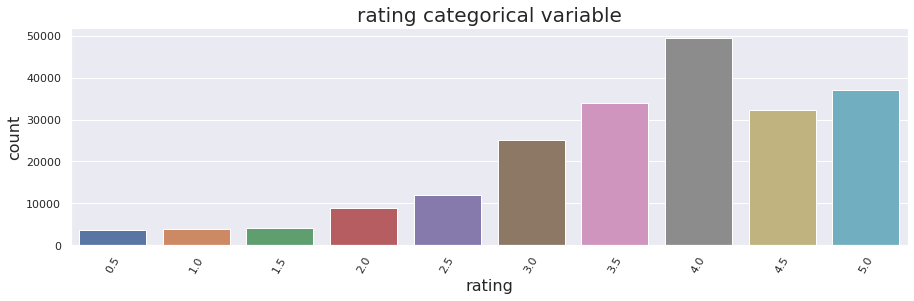
\includegraphics[width=15cm]{./images/rating-barplot.png}
	\caption{Este diagrama de barras expone la frecuencia o cantidad de observaciones para cada valor discreto de calificación o \textit{rating}.}
	\label{fig:ratingsBarPlot}
\end{figure}

En la figura~\ref{fig:ratingsBarPlot} se puede visualizar que el valor $4.0$
tiene la mayor frecuencia (moda), seguido de $5.0$ puntos y luego $3.5$ puntos.
Por otro lado, se debe tener en cuenta que estas calificaciones provienen de
todo los usuarios. Cada usuario tiene una forma propia de calificar, algunos
tienden a calificar de forma optimista, puntuando con valores altos, y otros
por el contrario, son mas pesimistas y tienden a puntuar con calificaciones
bajas. Este es un comportamiento conocido en el ámbito de sistemas de
recomendación. Se debe tener en cuenta que el valor $3.5$ para un usuario
podría ser un valor $4.5$ para otro. Por otro lado, se aprecia que en general
se tiende a puntuar valores a partir de $3.0$ punto en adelante, habiendo muy
pocas observaciones para puntuaciones menores a los $2.0$ puntos.

\clearpage

Para analizar en mas detalle la variable \textit{rating}, veamos a continuación
un histograma y \textit{boxplot} respectivamente:

\begin{figure}[h!]
	\centering
	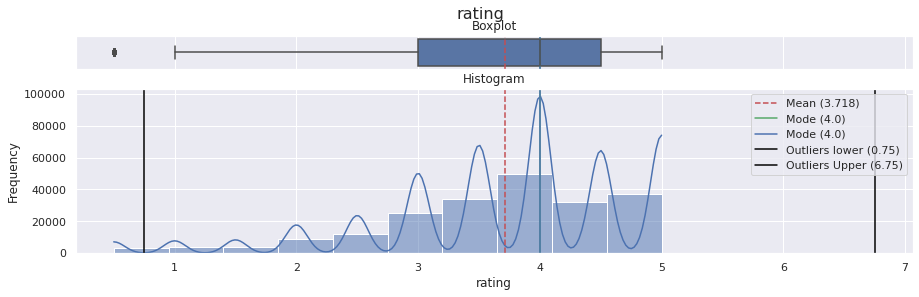
\includegraphics[width=15cm]{./images/rating-boxplot-histplot.png}
	\caption{Histograma y \textit{Boxplot} de la variable \textit{rating}. Los \textit{ratings} son las calificaciones realizadas por los usuario para cada ítem o película.}
	\label{fig:ratingsHistPlot}
\end{figure}

En la figura~\ref{fig:ratingsHistPlot} se aprecia que la variable
\textit{rating} tiene valores discretos entre $0.5$ y $5.0$ con un paso de
$0.5$. De esta forma, contamos con $10$ valores discretos de tipo real, siendo
claramente una variable categórica. Nuevamente vemos algo parecido al diagrama
de barras~\ref{fig:ratingsBarPlot}, el $50\%$ de las observaciones se
encuentran entre los cuantiles $Q1$ y $Q3$ con $3.0$ y $4.5$ puntos (Rango
inter-cuantil). La mediana (Cuantil $Q2$) esta claramente sobre los $4.0$
puntos, coincidiendo con la moda. La media se encuentra en los $3.5$ puntos a
izquierda de la mediana, debido a que tenemos puntos con frecuencia
considerables a izquierda que mueven a la media en esa dirección. Por otro
lado, tenemos valores atípicos en el extreme izquierdo en los $0.5$ puntos.
Esto se debe a que esta puntuación esta muy alejada del centro de los datos, el
cual se encuentra entre el cuantiles $Q1$ y $Q3$, donde tenemos el $50\%$ las
calificaciones con major probabilidad de ocurrencia. No se encuentran valores
atípicos por sobre el máximo. Se puede apreciar un sesgo a izquierda, ya que
existe mayor separación o dispersión de las observaciones entre $Q1$ y $Q2$ que
entre $Q2$ y $Q3$. De esta forma, ambos intervalos conservan su $25\%$ de las
observaciones pero hay menor dispersión entre $Q2$ y $Q3$.

\clearpage
A continuación segmentemos el anterior histograma por año:

\begin{figure}[h!]
	\centering
	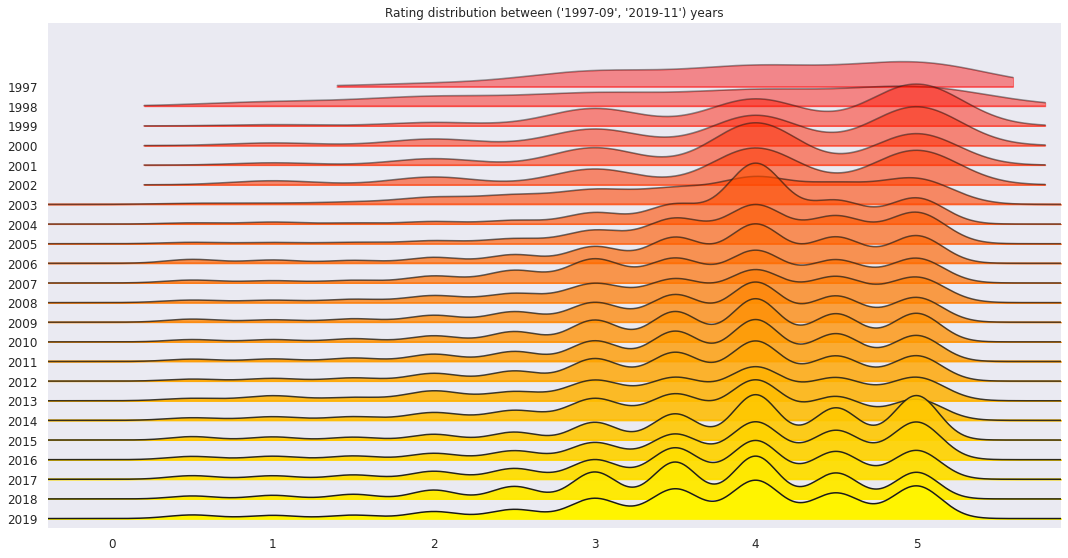
\includegraphics[width=15cm]{./images/rating-by-year.png}
	\caption{
		Histograma de calificaciones segmentado por año.
		Como aclaración, en esta gráfica se describen los histogramas
		como funciones densidad, a pesar de que la variable \textit{rating}
		es categóricas. De esta forma se puede apreciar con mas claridad
		la diferencia en cantidad de observaciones y el grado de dispersión de cada
		niveles por año.
	}
	\label{fig:ratingsYearHistPlot}
\end{figure}

En la figura~\ref{fig:ratingsYearHistPlot} inicialmente vemos que en los años
$1997$, $1998$ y $2003$ la curva tiende a ser mas lineal. Esto indica que la
forma de calificar es mas dispersa, es decir, no se encuentra un perfil de
puntuación claro por parte de los usuarios (si un item es un $4$ o un $5$ por
ejemplo). Entre $1999$ y $2022$ vemos que las puntuaciones $3$, $4$ y $5$ toman
mayor importancia siendo estas las mas utilizadas. Es decir, los usuarios
realizan en su mayoría puntuaciones en esos tres niveles. La mayor frecuencia
se puede ver claramente en los $4$ puntos en el año $2004$, donde fue
prácticamente la mas utilidades decayendo los $3$ y $5$ puntos, en comparación
a años anteriores. A partir del año $2005$ se nota un aumento cada vez más
demarcado en los niveles de puntuaciones entre los $3$ y $5$ puntos, donde los
usuarios cada vez más usan lo niveles $3.5$ y $4.5$. Debemos tener en cuenta
que el aumento en los niveles de puntuación con el tiempo, probablemente sean
debidos a un aumento año a año en la base de usuarios de \textit{Movie Lens} y
tal vez también sea el motivo por el cual en los primeros años vemos mucha
dispersion en las puntuaciones.

\clearpage

\subsection{Correlaciones}

Para realizar un analizar de correlación sobre todas la variables, se realizo
un \textit{merge}-\textit{join} de las tabla \textit{movies} e
\textit{interactions}, incluyendo solamente las columna numéricas. A
continuación podemos visualizar un diagrama de correlación de \textit{Pearson}
de las mismas:

\begin{figure}[h!]
	\centering
	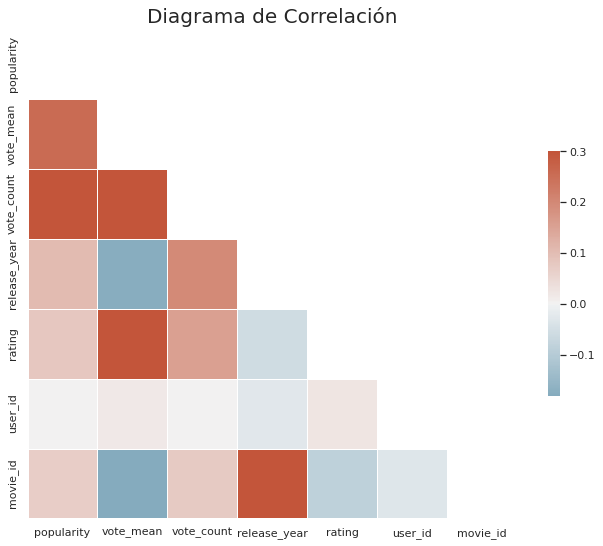
\includegraphics[width=9cm]{./images/Correlations.png}
	\caption{Diagrama de correlación de \textit{Person} aplicado a todas las variables numéricas resultado del \textit{merge} entre las tablas \textit{movies} e \textit{interactions}.}
	\label{fig:correlationPlot}
\end{figure}

En la figura~\ref{fig:correlationPlot} se aprecia de las variables
\textit{vote\_count}/\textit{vote\_mean} (Cantidad de votos/Media de votos) y
\textit{popularity} (Popularidad) tiene alta correlación debido a que las
películas mas votadas en general son las mas populares. Las variables
\textit{vote\_count} y \textit{vote\_mean} están altamente correlacionadas
entre si, ya que la media se calcula en base a la variable
\textit{vote\_count}. Por otro lado, también es de esperar que las
variables\textit{rating} (Calificaciones) y la \textit{vote\_mean} esten
correlacionadas, ya que a medida de aumenta la \textit{vote\_mean} tenemos
calificaciones mas altas. Se encuentra una alta correlación entre la variable
que identifica a una película y la variable \textit{relese\_year} (Fecha de
estreno). Esto se debe a que al momento de estrenarse una película, días
después a mas tardar, se da de alta la película en el sitio de \textit{Movie
	Lens}. Esto también nos dice que los \textit{ids} son secuenciales. Las
correlaciones en general son muy bajas llegando a $0.3$ como máximo. Esto es
una buena señal, ya que ayuda a diminuir el fenómeno de colinealidad de las
variables. Las variables que son combinaciones lineales de otras variables
puede producir que los modelos de \textit{Machine Learning} sobre-ajusten a los
datos de entrenamiento. Las variables \textit{vote\_mean} y \textit{movie\_id}
(Identificador de pelicula) tienen una correlación negativa muy baja. En algún
sentido nos dice que algunas películas mas nuevas tiende a tener una media de
votos menor. Lo mismo sucede entre las variables \textit{rating} y
\textit{movie\_id} en menor medida. Ambas con correlaciones negativas muy
bajas.

Si bien, en esta primera entrega no se están utilizando otras variables
distintas a \textit{user\_id} (id de usuario), \textit{movie\_id} y
\textit{rating}, es de interés analizar las variables correspondiente a
features de películas, ya que en el siguiente entrega (tesis) se planea
implementar modelos de recomendación híbridos, los cuales son ensambles de
sistemas de recomendación basados en contenido y filtros colaborativos.

\subsection{Variables de tipo texto}

Las variables de tipo texto son muy útiles para genera \textit{embeddings}, los
cuales se puede sumar o promediar, generando representaciones compactas de
ítems a recomendar. Luego es posible utilizar estas representaciones para
agrupar ítems según su sinopsis, \textit{tags}, título u otras variables como
pueden ser popularidad, año de estreno, votos, \textit{rating}, etc...

A continuación se puede visualizar la frecuencia de aparición de cada palabra
en cada uno de los campos de tipo texto. Cuanto mayor tamaño tenga la palabra
mayor frecuencia de aparición tendrá.

\begin{description}
	\item[Tags]
\end{description}

Cada usuario puede asociar \textit{tags} o palabras clase a una película. Un
\textit{tag} es una palabra o frase corta que identifica o describe una
película. Es una forma simple de clusterizar, ya que los usuarios en general
describen categorías como animación 3d, cual es el director, una frase que
describe algún tipo de categoría o algo relevante en el contenido de la misma.

\begin{figure}[h!]
	\centering
	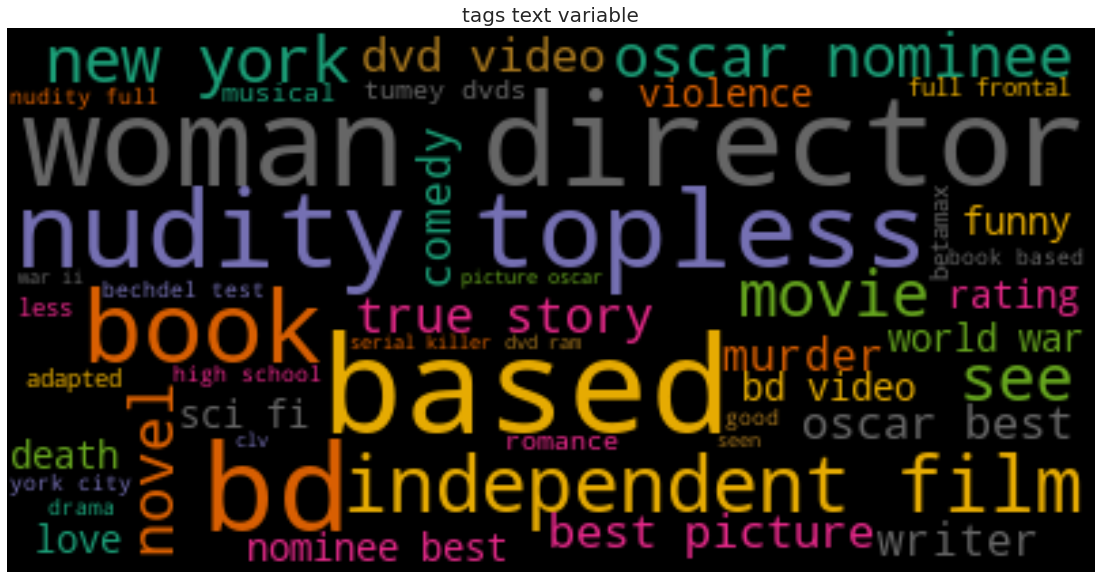
\includegraphics[width=9cm]{./images/Cloud-tags.png}
	\caption{Frecuencia de frases encontradas en la variable \textit{Tags}. El tamaño de cada frase representan la cantidad de apariciones de la misma.}
	\label{fig:tagsCloud}
\end{figure}

En la figura~\ref{fig:tagsCloud} las palabras \textit{based} (basada/o en),
\textit{Book}, \textit{Bd}, \textit{Director}, \textit{Nudity},
\textit{Topless}, \textit{Independent}, \textit{Film}, son aquella palabras mas
cargan por los usuarios en cada película. Otras palabras de menor frecuencia:
\textit{Movie}, \textit{Murder}, \textit{Novel}, \textit{Funny}, \textit{Oscar
	nominee}, \textit{Violent}, \textit{World war}, \textit{True story}.

\clearpage

\begin{description}
	\item[Overview]
\end{description}

La variable \textit{overview} es la sinopsis de la película. Esta describe
brevemente el contenido de la misma, sin revelar su desenlace.

\begin{figure}[h!]
	\centering
	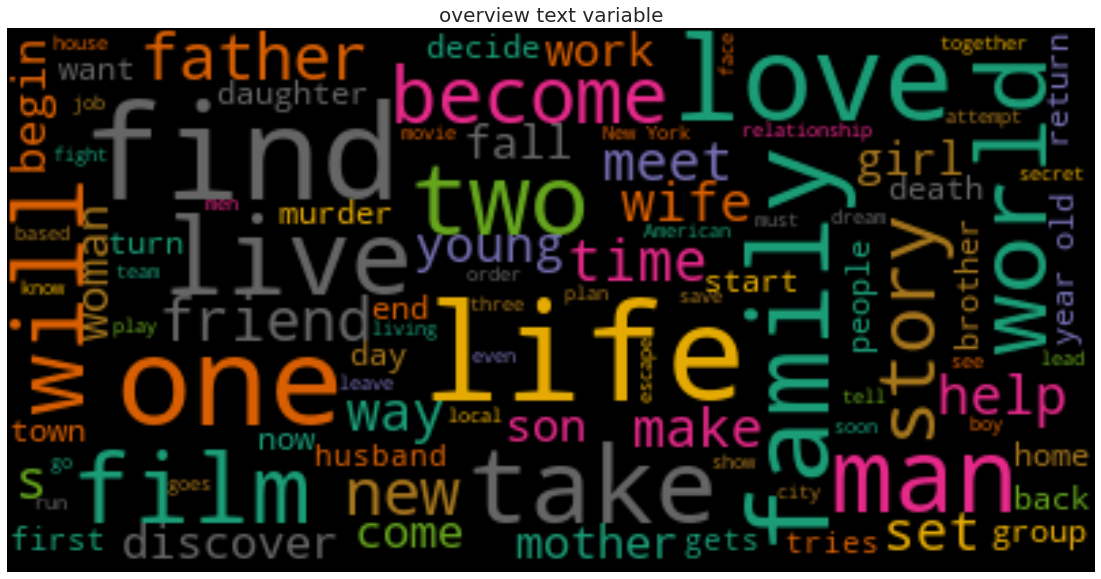
\includegraphics[width=9cm]{./images/Cloud-Overview.png}
	\caption{Frecuencia de palabras encontradas en la variable \textit{Overview}. El tamaño de cada palabra representan la cantidad de apariciones de la misma.}
	\label{fig:overviewCloud}
\end{figure}

En la figura~\ref{fig:tagsCloud} podemos visualizar las siguientes palabras con
mayor frecuencia: \textit{Find}, \textit{Live}, \textit{Love}, \textit{Wife},
\textit{One}, \textit{Man}, \textit{Film}, \textit{Become}, \textit{Family},
\textit{Story}, \textit{World}, \textit{Work}, \textit{Father}, \textit{New},
\textit{Friend} y \textit{Story}. Se aprecia una diferencia notoria entre las
variables \textit{tags} y \textit{overview}(Sinopsis). La variable
\textit{tags} parece categorizar las películas desde distintas perspectivas.
Por otro lado, la variable \textit{overview} contiene palabras que son mas
utilizadas en la descripción de la misma. A simple vista, los
clústers(\textit{Embeddings}) que pudieran generarse utilizando esta variable,
podrían ser mas específicos que aquellos \textit{clusters} generados a partir
de la variable \textit{tags}.

\begin{description}
	\item[Title]
\end{description}

\begin{figure}[h!]
	\centering
	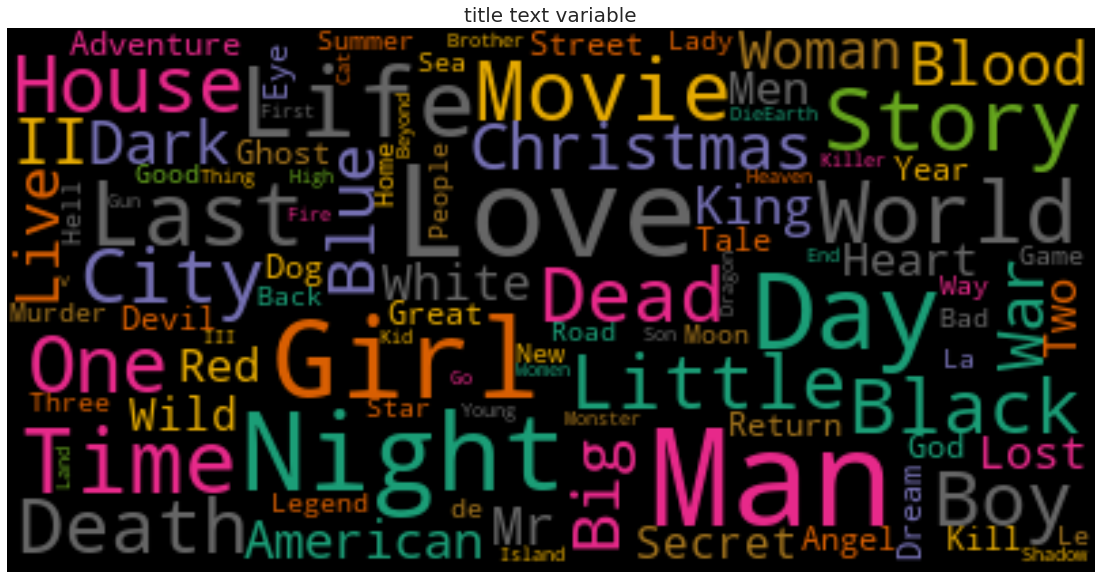
\includegraphics[width=9cm]{./images/Cloud-Title.png}
	\caption{Frecuencia de palabras encontradas en la variable \textit{Title}. El tamaño de cada palabra representan la cantidad de apariciones de la misma.}
	\label{fig:titleCloud}
\end{figure}

En la figura~\ref{fig:tagsCloud} podemos visualizar las siguientes palabras con
mayor frecuencia: \textit{Girl}, \textit{Man}, \textit{Day}, \textit{Dead},
\textit{Movie}, \textit{Time}, \textit{Night}, \textit{Life}, \textit{House},
\textit{Dark}, \textit{II}, \textit{Blood}, \textit{Christmas}, \textit{World},
\textit{War}, \textit{Black}, \textit{Boy}, \textit{Blue}, \textit{One} y
\textit{King}. A simple vista, una clusterización realizada con esta variable
puede ser mas general que la lograda con la variable \textit{overview}, pero
menos general que la variable \textit{tags}. En trabajos posteriores se
realizaran experimentos para ver resultado en este sentido.

\clearpage

\subsection{Análisis de Componentes Principales}

En esta sección se describe el análisis de componentes principales realizado
sobre las variable numéricas, resultado de fusionar las tablas \textit{movies}
y \textit{interactions}.

\begin{description}
	\item[Varianza Explicada]
\end{description}

Las componentes principales son las variables resultado al aplicar el algoritmo
\textit{PCA}~\cite{pca}. Estas nuevas variables tienen la particularidad de ser
ortogonales entre sí, lo que implica que no poseen ninguna correlación. Además,
a lo largo de todas las variables, la acumulación de varianza disminuye. Esto
indica que la primera componente tiene la mayor varianza y la última la menor
posible (en orden descendente).

\begin{figure}[h!]
	\centering
	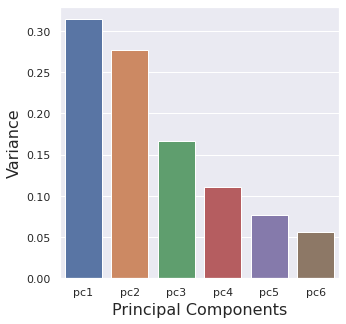
\includegraphics[width=8cm]{./images/PCA-Variance.png}
	\caption{Este diagrama de barras describe el grado de variabilidad o varianza explicada para cada componente principal resultado de aplicar el algoritmo\textit{PCA}~\cite{pca} sobre el conjunto de variables numericas originales.}
	\label{fig:explainedVariancePlot}
\end{figure}

\begin{description}
	\item[Varianza]
\end{description}
\begin{itemize}
	\item pc1: $31$ \%
	\item pc2: $28$ \%
	\item pc3: $16$ \%
	\item pc4: $11$ \%
	\item pc5: $7$ \%
	\item pc6: $5$ \%
\end{itemize}

En la figura~\ref{fig:explainedVariancePlot}, inicialmente podemos apreciar que
toda las componentes tiene niveles de variabilidad o varianza explicada muy
bajos, donde la primera componente llega solamente al $31$ \%. Esto indica que
el grado de correlación de las variables originales es muy bajo. Utilizando el
citerio del bastón roto podríamos seleccionar las 3 primeras componentes
principales, ya que son las que acumulan mayor varianza.

Por otro lado, debemos tener en cuenta que el análisis por componentes
principales es un análisis lineal. Es decir, tiene encuentra unicamente
correlaciones lineales entre las variables originales. De esta forma, el método
puede estar perdiendo de vista correlaciones no lineales mas complejas, donde
podríamos encontrar un mayor grado de correlación. Las 3 primeras componentes
acumulan un grado de variabilidad del $85$ \%.

\begin{description}
	\item[Cargas o Loadings]
\end{description}

Las componentes principales son combinaciones lineales de las variables
originales. Luego, las cargas o \textit{loadings} son los coeficientes
utilizados para transformar las variables originales en las componentes
principales mediante combinaciones lineales.

De esta forma, los coeficientes definen una medida de correlación o grado de
aporte de cada variable original a una componente principal.

A continuación se pueden visualizar las cargas o \textit{loadings}:

\begin{table}[h!]
	\centering
	\begin{tabular}{lrrrrrr}
		\toprule Variable   & PC1    & PC2   & PC3     \\
		\midrule Popularity & 0.79   & -0.09 & -0.003  \\
		Vote Mean           & 0.55   & -0.55 & -0.03   \\
		Vote Count          & 0.88   & -0.11 & -0.0002 \\
		Release Year        & 0.33   & 0.8   & 0.045   \\
		User ID             & -0.006 & -0.08 & 0.99    \\
		Movie ID            & 0.24   & 0.8   & 0.04    \\
		\bottomrule
	\end{tabular}

	\caption{Coeficientes de componentes principales vs. variables originales. Cada uno de estos valores representan el grado de correlación o aporte de cada variable original a cada componente principal.}

	\label{fig:loadingsTable}
\end{table}

En la tabla~\ref{fig:loadingsTable} vemos que \textit{Vote Count (88\%)}
(Cantidad de votos) y \textit{Popularity (80\%)} (Popularidad) tiene una
correlación positiva muy alta sobre la componente $PC1$. Lo mismo sucede con
\textit{Vote Mean (55\%)} (Media de la cantidad de votos) en menor medida.
Entre dos observaciones con distintos valores de popularidad, la que tenga un
valor mas alto, aportara mas a la componente $PC1$ que a las otra dos ($PC2$ y
$PC3$). También vemos que las variable \textit{Release Year} (Año de estreno) y
\textit{Movie ID} tienen un aporte, considerable, pero mas bajo del 33\% y 24\%
respectivamente, sobre la componente $PC1$. La variable \textit{User ID} no
tiene aporte alguno sobre la componente $PC1$. Las variables que mas aportan a
la componente $PC2$ son \textit{Vote Mean (55\%)} y \textit{Vote Count (11\%)}
respectivamente. Este aporte es negativo, esto indica que un aumento en los
niveles de esta variable significa una disminución en la componente $PC2$. La
variable \textit{Release Year} (Año de estreno) tiene el aporte positivo mas
alto sobre la componente $PC2$ siendo del 80 \%. Para la componente $PC3$, las
variables que mas aportan son \textit{User ID (99\%)} y \textit{Release Year
	(45\%)} respectivamente, ambas positivas. Vemos que un aumento en la variable
\text{User ID} produce un aumento casi en una unidad sobre el coeficiente, pero
\textit{Release Year} es la mitad en relación. De este forma, la componente
$PC1$ podríamos nombrarla como Nivel de popularidad o conocimiento general de
una película. La componente $PC2$, en algún sentido mide lo contrario a la
popularidad, es un indicador de cuan \textit{underground} es un nuevo estrenos.
La componente $PC3$ es mas difícil de nombrar, pero podría llamarse: Grado
\textit{newbie} de un usuario, indicando cuan nuevo es un usuario.

\clearpage

\begin{description}
	\item[\textit{Biplot}]
\end{description}

\begin{figure}[h!]
	\centering
	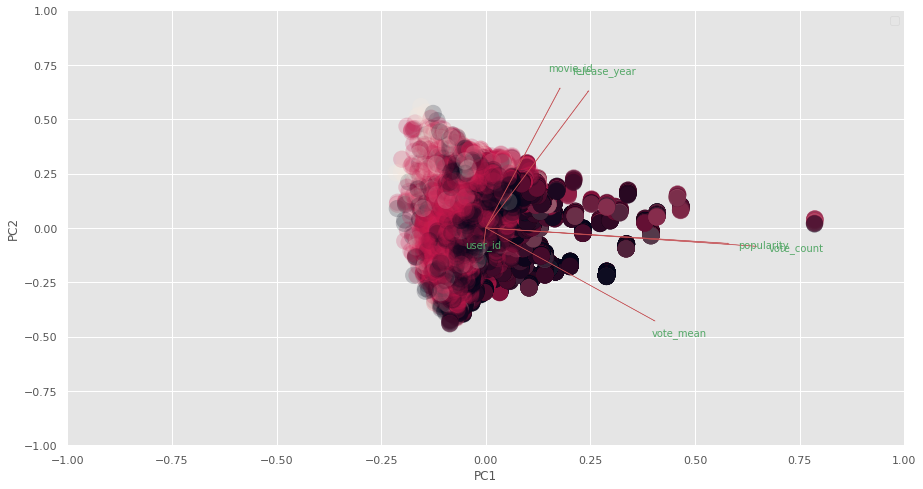
\includegraphics[width=15cm]{./images/PCA-biplot.png}
	\caption{Diagrama~\cite{biplot}\textit{Biplot}. Este diagrama representa los valores de
		las variables originales coloreados en color rojo, negro y gris.
		Estos colores corresponden a tres segmentos de calificaciones: $>2$, entre $2$ y $3.5$ y $>4$. También se pueden apreciar los vectores correspondientes a las variables originales.}
	\label{fig:biplot}
\end{figure}

En la figura~\ref{fig:biplot} se expone un diagrama
\textit{Biplot}~\cite{biplot}. Este representa los valores de las variables
originales coloreados en color rojo, negro y gris correspondientes a tres
segmentos de calificaciones: $>2$, entre $2$ y $3.5$ y $>4$. También se
representan los vectores correspondientes a las variables originales. A primera
vista observamos que las variables \textit{Popularity} (Popularidad) y
\textit{Vote Count} (Cantidad de votos) tienen una correlación muy alta, ya que
el ángulo entre sus vectores es prácticamente cero. Esto tiene sentido, ya que
ambas son medidas de popularidad de alta colinealidad. Las variables
\textit{Popularity} (Popularidad), \textit{Vote Count} (Cantidad de votos) y
\textit{Vote Mean} (Media de la cantidad de votos) tiene un aporte positivo
sobre la componente $PC1$ (En menor media). Esto último se corresponde con los
coeficientes de las cargas analizados anteriormente. Las variables
\textit{Movie ID} y \textit{Release Year} (Año de estreno) aportan en menor
medida sobre la componente $PC1$. De esta forma, se constata lo visto
anteriormente en análisis de carga, donde la componente $PC1$ representa el
grado de popularidad de una película. La variable \textit{Vote Mean} (Media de
la cantidad de votos) aporta en forma negativa y las variables \textit{Movie ID
} y \textit{Release Year} (Año de estreno), en forma positiva sobre la
componente $PC2$. Las varaibles \textit{Popularity} (Popularidad), \textit{Vote
	Count} (Cantidad de votos) tienen casi aporte nulo a la componente $PC2$ en
correspondencia con el analisis de cargas anteriormente expuesto. Si
visualizamos los puntos que representan a las observaciones originales en el
espacio latente generado por \textit{PCA}~\cite{pca}, vemos que las
observaciones de color negro ($>4$ puntos) y gris (entre $2$ y $3.5$ puntos) se
encuentran mas a la derecha que aquellas coloreadas en rojo ($>2$ puntos). Esto
indica que hay un crecimiento del nivel de popularidad cuanto mas a derecha se
encuentre un punto en la componente $PC1$, validando los análisis anteriores.
Si visualizamos lo puntos correspondientes a las observaciones en las
direcciones de la componente $PC2$, vemos que a major valor en la componente,
menor es el grado de popularidad de las películas, ya que los puntos rojos
tienden a estar en el extremo positivo de la componente. Esto valida la
hipótesis de que la componente $PC2$ indica cuan \textit{underground} es un
película.

\chapter{Métodos}

En este capitulo se describirán los modelos utilizados para realiza la
predicción de la clasificación de un usuario para una película que aun no ha
visto. Para realizar esto, se utilizaron varios modelos basados en filtros
colaborativos.

Cada implementación tiene sus particularidades: Su nivel de escalabilidad, sus
tiempos de entrenamiento y predicción, su implementación, la exactitud de las
predicciones, su tendencia al sobre ajuste, etc.. Para este trabajo se
eligieron dos grandes grupos. Por un lado, una implementación sencilla basada
en memoria, como es el algoritmo de K vecinos cercanos. Por otro lado, modelos
basados en \textit{Deep Learning}. Los modelos basados en \textit{Deep
	Learning} utilizan \textit{Embeddings} en todos los casos, como una forma de
reducir la dimensionalidad de las variables categóricas que se utilizan como
entradas al modelo. Además, cada modelo tiene su propia arquitectura, algunas
clásicas y otras basadas en modelos del estado del arte. Luego, la idea fue
medir los resultados de todo los modelos, utilizando distintas métricas
comparables, entrenando con el mismo \textit{dataset} en todos los casos. De
esta forma podemos comparar los resultados de todos los modelos. Como
\textit{baseline} se tomo el modelo de K vecinos cercanos (\textit{KNN}), dado
que es el modelo mas simple. Este servira como punto partida para comparar
resulados con otros modelos mas complejos.

Por otro lado, dada la cantidad de datos con la que se cuenta y teniendo en
cuenta que estos modelos son muy demandantes en cuanto a recursos de
\textit{hardware}, se opto por usar el framework
\href{https://pytorch.org/}{\textit{PyTorch}}. Dado que permite hacer uso tanto
de \textit{CPU} como \textit{GPU}. De esta forma, se puede elegir cuando usar
cada dispositivo y en que parte del flujo (pre-procesamiento, entrenamiento e
inferencia). Ya elegido el \textit{framework}, se opto por implementar todos
los modelos desde sus bases, ya que \textit{PyTorch} no cuenta con mucho
modelos del estado del arte desarrollados de forma oficial. De esta forma se
implemento cada modelo desde cero para poder hacer uso de \textit{CPU} y
\textit{GPU} de forma granular y realizar un uso mas eficiente de los recursos
disponible. Mas adelante veremos que esto puede inpactar fuertemente en los
tiempos de entrenamiento e inferencia.

\section{Enfoque Basados en Memoria}

\subsection{Algoritmo de los K vencinos cercanos (\textit{K-Nearest-Neighbor} o \textit{KNN})}

Esta es la implementación clásica y mas intuitiva para realizar recomendación
de ítems. Una vez entrenado el modelo, se cuenta con una matriz de distancias
que pueden ser: distancias entre usuarios o ítems, y otra matriz de
calificaciones usuario-ítem. De esta forma, en la etapa de inferencia, el
modelo toma como entrada un usuario (\textit{user\_id}) y un ítem
(\textit{item\_id}) y retorna la predicción de la calificación. Estas matrices
se puede mantener en memoria, persistir en una base de datos (como puede ser
\textit{Redis}) o en un archivos indexado. Por esta cuestión, la categoría en
memoria no tiene por que ser estricta, pero si se entiende que los mejores
tiempos de inferencia y entrenamiento se lograran cuando se tenga parte o la
totalidad de estas matrices en memoria.

\clearpage

Luego, para realizar el entrenamiento del modelo se necesita una lista de
tuplas, donde cada tupla contiene:

\begin{description}
	\item[Lista de tuplas]
\end{description}
\begin{equation}
	Tuplas = [<u_1; i_1; r_{u_1, i_1}>,...,<u_n; i_m; r_{u_n, i_m}>]
\end{equation}
\begin{description}
	\item[Donde:]
\end{description}
\begin{itemize}
	\item $u$ es un identificador secuencial, univoco y numérico de un usuario. Estos identificadores se generan a partir de una secuencia numérica, es decir que no debemos tener huecos para minimizar el uso de memoria en caso de no usar matrices ralas.
	\item $i$ es un identificador secuencial, univoco y numérico de un ítem. En este caso los ítems son películas, pero podrían ser cualquier entidad identificable como productos, usuarios, comidas, etc..
	\item $r_{u, i}$ es la calificación otorgada al ítem $i$ por parte del usuario $u$.
	\item $n$ es la cantidad total de usuarios en el \textit{dataset} de entrenamiento.
	\item $m$ es la cantidad total de ítems en el \textit{dataset} de entrenamiento.
\end{itemize}

Dada esta lista de tuplas, podemos construir una matriz esparza donde cada fila
representa a un usuario y cada columna a un ítem o vise versa, y las celdas o
valores de la misma contienen las calificaciones.

\begin{description}
	\item[Matriz de calificaciones]
\end{description}
\begin{equation}
	Calificaciones_{u,i} =
	\begin{pmatrix}
		r_{1,1} & r_{1,2} & \cdots & r_{1,i} \\
		r_{2,1} & r_{2,2} & \cdots & r_{2,i} \\
		\vdots  & \vdots  & \ddots & \vdots  \\
		r_{u,1} & r_{u,2} & \cdots & r_{u,i}
	\end{pmatrix}
\end{equation}

\begin{description}
	\item[Donde:]
\end{description}
\begin{itemize}
	\item $r_{u,i}$ es la calificación otorgada al ítem $i$ por parte del usuario $u$.
	\item Cada vector fila $F_u$ contiene todas la calificaciones realizadas por el
	      usuario $u$ para todos los ítems. Los ítems que aun no tiene calificación
	      contiene el valor $0$.
	\item Cada vector columna $C_i$ contiene las calificaciones realizadas por todos los
	      usuarios para el ítem $i$. Las posiciones correspondientes a los usuarios que
	      aun no calificaron el ítem $i$ tendrán el valor $0$.
\end{itemize}

En el siguiente paso, se debe construir la matriz $Distancias_{u_a,u_b}$ que
contiene las distancias entre todos los vectores fila $F_u$ de la matriz de
$Calificaciones_{u,i}$. Cabe aclarar que cada vector fila $F_u$ de la matriz de
$Calificaciones_{u,i}$ representa a un usuario, ya que contiene todas las
calificaciones realizadas por el mismo.

\clearpage
\begin{description}
	\item[Matriz de distancias]
\end{description}
\begin{equation}
	Distancias_{u_a,u_b} =
	\begin{pmatrix}
		d_{1,1}   & d_{1,2}   & \cdots & d_{1,u_b}   \\
		d_{2,1}   & d_{2,2}   & \cdots & d_{2,u_b}   \\
		\vdots    & \vdots    & \ddots & \vdots      \\
		d_{u_a,1} & d_{u_a,2} & \cdots & d_{u_a,u_b}
	\end{pmatrix}
\end{equation}

\begin{description}
	\item[Donde:]
\end{description}
\begin{itemize}
	\item $d_{u_a,u_b}$ es la distancia entre el vector fila $F{u_a}$ y $F{u_b}$ de la matriz de $Calificaciones_{u,i}$.
\end{itemize}

En cuanto a las distancias, no hay una restricción acerca de cual utilizar. En
general las distancias que mejor ajustan apra este dominio son las siguientes:

\begin{itemize}
	\item Distancia Coseno Ajustado.
	\item Distancia Coseno.
	\item Distancia de \textit{Pearson} (1 - Correlación de \textit{Pearson}).
\end{itemize}

Luego, para este trabajo se eligió utilizar la distancia coseno.

\begin{description}
	\item[Distancia Coseno]
\end{description}

La distancia coseno es una medida de similitud entre dos vectores en un espacio
vectorial que posee un producto interno. La distancia coseno entre dos vectores
se mide en grados. De esta forma, cuanto menor es el ángulo entre dos vectores
mas similares son entre sí. De forma contraria, cuando mayor es el ángulo entre
dos vectores menos similares seran. A contunaicon se define la distancia coseno
como:

\begin{equation}
	Distancia \mspace{3mu}Coseno_{ua, ub} = \frac{ \sum_{i \in I} r_{ua, i}.r_{ub, i}}{\sqrt{\sum_{i \in I} r_{ua, i}^2}.\sqrt{\sum_{i \in I} r_{ub, i}^2}  }, ua \neq ub
\end{equation}

\begin{description}
	\item[Donde:]
\end{description}
\begin{itemize}
	\item $ua$ y $ub$ son los indices de dos vectores fila $F_u$ de la matriz de $Calificaciones_{u,i}$. Cada uno de estos vectores fila $F_u$ representan a un usuario.
	\item $ua \neq ub$, es decir que cada índice representa a un usuario distinto.
	\item $I$ es la cantidad total de columnas de la matriz de $Calificaciones_{u,i}$.
	\item $i$ el índice de una columna de la matriz de $Calificaciones_{u,i}$. Cada columna representa a un ítem y contiene todas las calificaciones realizadas por todos los usuarios sobre el ítem $i$.
	\item $0 <= Distancia \mspace{3mu} Coseno_{ua, ub} <= 1$. Cuanto menor sea el valor de $Distancia \mspace{3mu} Coseno_{u_a, u_b}$ mas similares serán los usuarios con los indices $u_a$ y $u_b$.
\end{itemize}

\clearpage
\begin{description}
	\item[Similitud Coseno]
\end{description}
\begin{equation}
	Similitud \mspace{3mu}Coseno_{ua, ub} = 1- Distancia \mspace{3mu}Coseno_{ua, ub}
\end{equation}
\begin{description}
	\item[Donde:]
\end{description}
\begin{itemize}
	\item $0 <= Similitud \mspace{3mu}Coseno_{ua, ub} <= 1$. Cuanto mayor sea el valor de $Similitud \mspace{3mu}Coseno_{ua, ub}$ mas similares serán los usuarios con los indices $u_a$ y $u_b$.
\end{itemize}

Volviendo a nuestro algoritmo, la idea es calcular la distancia de cada vector
fila $F_u$ de la matriz de $Calificaciones_{u,i}$ contra todos los demás
vectores fila de la misma matriz, obteniendo asi la matriz de
$Distancias_{u_a,u_b}$, donde cada fila y columnas representa a los vectores
fila $F_u$ de la matriz de $Calificaciones_{u,i}$.

Aquí es donde finaliza la etapa de entrenamiento. Luego la inferencia o
predicción depende de la implementación que se elige para predecir las
calificaciones. En todos los casos se utilizan ambas matrices para realizar las
predicciones. A continuación una explicación del paso de inferencia o
predicción para cada implementación elegida.

\clearpage

\subsection{Algoritmo de los K vencinos cercanos basado en usuarios (\textit{KNN User Based})}

En el apartado anterior se explico cómo calcular las matrices de
$Calificaciones_{u,i}$ y $Distancias_{u_a,u_b}$. El cálculo de estas matrices
es parte del proceso de entrenamiento del modelo \textit{KNN}. En este apartado
se explicará el proceso para realizar la predicción o inferencias de la
calificación de un ítem por parte de un usuario~\cite{useritembasedinference}.

Entonces, el enfoque de K vecinos cercanos para predecir la calificación de un
ítem, se basa en la siguiente definición:

\begin{equation}
	Prediccion \mspace{3mu}basada \mspace{3mu}en \mspace{3mu}usuarios\mspace{3mu}_{u, i} = \overline{r}_{u} + \frac{\sum_{o \in O} (r_{o, i} - \overline{r}_o) . w_{u, o} }{ \sum_{o \in K} w_{u, o}}, u \neq o
\end{equation}

\begin{description}
	\item[Donde:]
\end{description}
\begin{itemize}
	\item $Prediccion \mspace{3mu}basada \mspace{3mu}en \mspace{3mu}usuarios\mspace{3mu}_{u, i}$ es la predicción de la calificación del usuario $u$ para el ítem $i$.
	\item $o$ (Minúscula) pertenece al conjunto $O$ (Mayúscula) de usuarios. $O$ es el conjunto de todos los usuarios menos el usuario $u$.
	\item $w_{u,o}$ es la similitud entre los usuarios $u$ y $o$. Se calcula mediante $Similitud \mspace{3mu}Coseno_{u, o}$
	\item $u \neq o$, es decir que cada índice representa a un usuario distinto.
	\item $\overline{r}_{u}$ es el promedio de todas las calificaciones realizadas por el usuario $u$. Se pueda calcular como $\overline{r}_{u} = \frac{1}{N} \sum_{i=1}^N Calificaciones_{u,i}$, siendo $N$ el la cantidad de total de ítems.
	\item $r_{o,i} - \overline{r}_{o}$ es la diferencia entre la calificación del usuario $o$ para el ítem $i$ y el promedio de calificaciones del usuario $o$. Esta diferencia se utiliza para ajustar el sesgo de calificación de cada usuario. Este sesgo se da debido a la subjetividad que tiene cada usuario al momento de calificar un ítem. Algunos usuarios tienden a calificar todo de forma optimista, otorgando calificaciones mas bien altas; otros usuarios son mas pesimistas y tienden a poner calificaciones bajas. Al restar por la medio de calificación de cada usuario, estamos normalizando las calificaciones, haciéndolas mas o menos comparables, siendo esta una forma de disminuir este fenómeno de subjetividad al momento de calificar un ítem.
\end{itemize}

Finalmente, a grandes rasgos, el calculo de la predicción no es mas que el
promedio de calificaciones del usuario $u$ sumado al promedio pesado de las
calificación de los demás usuarios para el ítem $i$, donde los pesos son las
distancias del usuario $u$ con los demás usuarios.

Ahora, por un tema performance el conjunto $O$ no contiene a todos los demás
usuarios, sino un conjunto de tamaño $K$ el cual contiene a los usuario mas
cercanos en términos de distancia. Es decir que, como paso previo a la
predicción, es necesario encontrar a los $K$ usuarios mas cercanos al usuario
$u$. De esta forma, el parámetro $K$ se convierte en un hiper-parámetro del
modelo. Luego a mayor $K$, mayor sera número de vecinos a tener en cuenta para
calcular la predicción, y mayor será el tiempo de inferencia del modelo. Por
otro lado, a mayor $K$ estaremos incluyendo mas vecinos que son menos similares
en términos de distancia. Debido a esto, siempre se busca encontrar el mejor
valor posible para $K$. Este valor se buscado a través de una optimización de
hiper parámetros regida por una métricas que valide la exactitud del modelo al
momento de la predicción, obteniendo como resultado el $K$ para el cual el
modelo tiene el resultado mas exactos posibles.

\subsection{\textit{KNN Item Based}}

Este modelo es muy similar al anterior, la diferencia radica en que la matriz
de $Calificaciones_{i, u}$ tiene ítems como filas en vez de usuarios, y
usuarios como columnas en vez de ítems. Es decir, es la matriz transpuesta de
la matriz de $Calificaciones_{u, i}$ original~\cite{useritembasedinference}. De
esta forma, la matriz de $Distancias_{i_a,i_b}$ mide las distancia entre
vectores fila $F_i$ los cuales representan ítems. Por otro lado, también
existen diferencias con el modelo anterior, al momento de calcular las
predicciones. A continuación la definición del calculo de las predicciones:

\begin{equation}
	Prediccion \mspace{3mu}basada \mspace{3mu}en \mspace{3mu}items\mspace{3mu}_{u, i} = \frac{\sum_{o \in O} r_{u, o}. w_{i, o} }{\sum_{o \in O} w_{i, o} }, i \neq o
\end{equation}
\begin{description}
	\item[Donde:]
\end{description}
\begin{itemize}
	\item $Prediccion \mspace{3mu}basada \mspace{3mu}en \mspace{3mu}items\mspace{3mu}_{u, i}$ es la predicción de la calificación del usuario $u$ para el ítem $i$.
	\item $O$ es el conjunto de los vecinos cercanos o mas similares de $i$ previamente seleccionado. $o$ pertenece al conjunto $O$.
	\item $i \neq o$: los indices ítem $i$ y $o$ representan a ítems distintos.
	\item $w_{i,o}$ es la similitud entre los ítems $i$ y $o$.
\end{itemize}

Finalmente la predicción, un promedio pesado de las calificaciones del usuario
$u$ para los ítems vecinos al ítem $i$, pesadas por la similitud de cada ítem
$o$ con $i$.

\subsection{\textit{KNN User Based Ensemble} y \textit{Item Based}}

Dado que contamos dos modelos basados en \textit{KNN} se realizo un sample de
ambos modelos el cual realiza un promedio de las salidas de ambos modelos.

\section{Enfoque basado en modelos}

Hasta aquí realizamos una descripción del modelo \textit{KNN} utilizados en
este trabajo y las distintas implementaciones utilizadas. Estos modelos tiene
varias falencias. Entre las mas importantes encontramos el problema de escala,
ya que el tamaño de los datos a procesar depende casi linealmente de los
recursos de memoria, \textit{CPU} y/o \textit{GPU} disponibles. De esta forma,
cuando es necesario procesar una gran cantidad de datos para realizar
predicciones, se opta por modelos que realicen algún tipo de reducción de
dimensionalidad para construir su representación internal, la cual luego se
utilizada para realizar las predicciones. A esta presentación interna muchas
veces se la llama modelo, ya que el modelo en si no es el algoritmo utilizado
si no el estado internal al que se llega luego del entrenamiento.

\subsection{\textit{One-Hot Encoding vs. Embeddings}}

Particularmente en el ámbito de recomendaciones, se cuenta con variables
categóricas de alta dimensionalidad. Para este trabajo, tenemos dos variable
con esta característica: los ids secuenciales de usuarios e ítems. Cuando
trabajamos con modelos de Machine Learning, particularmente con redes
neuronales, es necesario convertir las variable categóricas en una
representación numérica. El enfoque mas simple o native es realizar un one-hot
encoding de la variable categórica, el cual consta de codificar cada posible
valor de la variable como un vector que contiene tantas posiciones como valores
tenga la variable. De esta forma, cada vector tiene un 1 en la posición que
concuerda con el valor representado y un cero en las demás posiciones. Por
ejemplo, suponemos que tenemos la siguiente variable:

\begin{itemize}
	\item Variable Categórica: Estado del Tiempo.
	\item Posibles valores: Nublado, Despegado y Lluvioso.
\end{itemize}

Si codificamos sus valores usando \textit{one-hot encoding} obtenemos lo
siguientes vectores:

\begin{itemize}
	\item $Nublado    = [1, 0, 0]$
	\item $Despegado  = [0, 1, 0]$
	\item $Lluvioso   = [0, 0, 1]$
\end{itemize}

Entonces, el valor \textit{Nublado} se convierte en 3 entradas para una red
neuronal a las cuales se le pasa los numero $1$, $0$ y $0$ respectivamente.
Ahora pensemos en la cantidad de usuarios que tiene \textit{Google} o
\textit{Amazon}, ¿Que tamaño tendría el vector que representa a un solo
usuario?¿Por qué usar un vector 99\% ralo para representar un valor?¿No hay una
forma mas compacta de realizar esta codificación?

La respuesta corta es sí, en estos casos se utilizan \textit{Embeddings}. ¿Pero
que son los \textit{Embeddings} y en que se diferencian de la codificación
\textit{one-hot}?

Un \textit{Embedding} no es mas que una forma de codificar valores de una
variable categórica usando vectores de menor tamaño. Es decir, si tenemos una
variable categórica que tiene 10.000 posible valores, dependiendo del caso,
podríamos elegir un tamaño de 100 posiciones. Este tamaño debe ser elegido de
forma tal que no se produzca pérdida de información. Por esta cuestión, el
tamaño de estos vectores se transforma en un hiper-parámetro mas a ajustar al
momento de entrenar los modelos que utilicen esta técnica de codificación.

Otro punto importante que diferencia ambas codificaciones, reside en la
distancia entre vectores. Si tomamos dos vectores con codificación
\textit{one-hot} y los gráficas en un espacio tridimensional o bidimensional,
se aprecia que el ángulo entre estos siempre es el mismo, 90 grados. Supongamos
el caso anterior de la variable \textit{Estado del Tiempo}, si representamos en
el espacio todos sus valores, podemos ver que la distancia es las misma entre
cualquier par de vectores. Si ahora codificamos la misma variable usando
\textit{Embeddings} esto cambia, ya que los vectores que representan a los
valores \textit{Nublado} y \textit{Lluvioso} tiene un ángulo menor a 90 grados.
Por otro lado, ambos vectores están alejados del vector \textit{Despejado}. De
esta forma un \textit{Embedding} permite captar mas información ya que realiza
una clusterización de los valores que son mas cercanos en términos de
significado. Los días nublados y lluviosos son muy parecido entre sí y muy
distintos a un dia despejado.

De esta forma los \textit{embeddings} tiene una doble ganancia sobre la
codificación \textit{One-Hot}: comprimen la información y además captan
información útil para la clusterización de sus valores. Algo interesante a
destacar es que los modelos que entrenan \textit{Embeddings} captan esta
información de forma automática en base a las observaciones usadas en el
entrenamiento, generando estos espacios latentes llamados \textit{Embeddings}.

\subsection{\textit{Embedding Layer}}

En el ámbito del \textit{Deep Learning} o \textit{Machine Learning} se cuenta
con la abstracción de \textit{Capas} (\textit{Keras/Tensorflow}) o
\textit{Módulos} (\textit{PyTorch}), las cuales encapsulan el comportamiento
esencial en un conjunto de bloque básicos utilizados para construir cualquier
modelo. Los bloques que permiten que un modelo infiera o construya un
\textit{embedding} durante el entrenamiento son los bloques
\textit{Embedding/EmbeddingBag} en \textit{PyTorch} o \textit{Embedding} en
\textit{Keras/Tensorflow}. En ambos \textit{frameworks} el comportamiento del
estos bloques es el mismo.

Por un lado, podemos elegir el tamaño de los vectores \textit{embedding}, el
cuál, como ya adelantamos, es un hiper-parámetro mas a optimizar. Por otro
lado, debemos definir la cantidad de vectores \textit{embedding} que debe
contener la capa. Ésta es siempre igual al número total de valores que puede
tomar variable categórica.

De esta forma, para crear una capa o módulo \textit{Embedding} para la variable
\textit{Estado del Tiempo} podríamos crear una capa \textit{Embedding} de
tamaño 3, ya que cuenta con 3 posible valores, con un tamaño de vector siempre
menos a 3, ya que de lo contrario tendríamos la misma dimensionalidad que
tenemos al usa la codificación \textit{one-hot}, con la diferencia de que una
capa \textit{Embedding} capta la similitud entre los valores de la variable
categórica un la codificación \textit{one-hot} no.

Luego el modo de funcionamiento de la capa es muy simple. Esta se puede pensar
como una tabla \textit{Hash}. donde cada clave es un valor de la variable
categórica. Es decir, que tendremos tantas claves como valores pueda tomar la
variable categórica. Estas claves son codificados a números y los valores
asociados a cada clave son vectores \textit{embedding}. Cave aclarar que en
general, estos vectores son inicializados con valores aleatorio. Luego, el
modelo irá ajustando los valores de cada vector \textit{embedding} durante el
proceso de entrenamiento.

En el \textit{froward pass}, como entrada se pasa un valor codificado a números
de la variable categórica. Para nuestra variable \textit{Estado del Tiempo}
podríamos codificar sus valores como sigue: \textit{Nublado = 0},
\textit{Despegado = 1}, \textit{Lluvioso = 2}.

Entonces si pasamos el valores \textit{Nublado} como entrada a la capa, en
realidad estamos pasando la clave 0. Luego, de esto la capa resuelve el vector
\textit{embedding} asociado a esa clave y lo devuelve a su salida.

Finamente, debemos tener en cuenta que el proceso de \textit{back-propagation}
sera el encargado de ir ajustando los valores, también llamados pesos de los
vectores \textit{embedding}, de acuerdo a lo que se requiera en la salida del
modelo, durante el proceso de optimización de descenso del gradiente.

\begin{figure}[ht!]
	\centering
	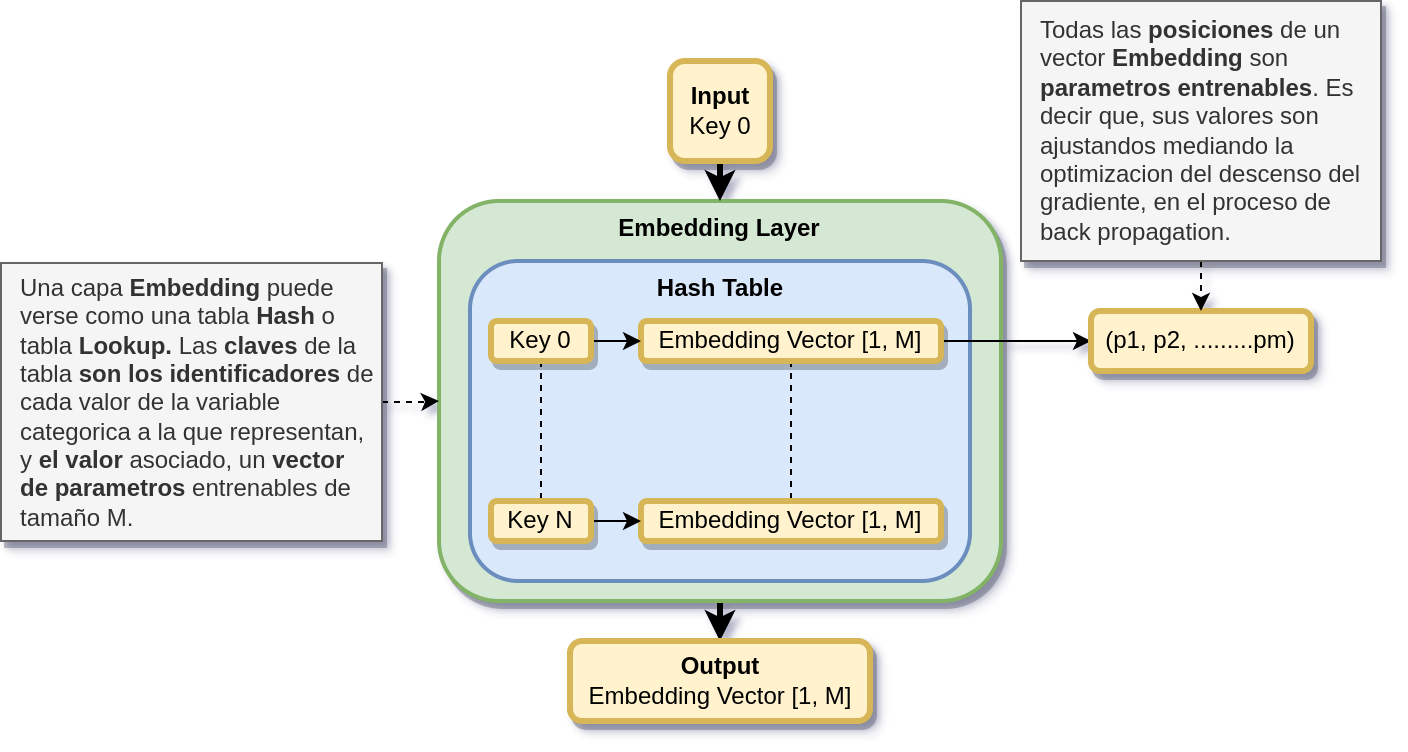
\includegraphics[width=13cm]{./images/Embedding-Layer.png}
	\caption{Esquema de una capa o módulo \textit{Embedding}.}
	\label{fig:embeddingLayer}
\end{figure}

\clearpage

\subsection{Arquitecturas Utilizadas}

En la sección anterior se explicó uno de los componentes básicos y más
utilizados en los modelos de recomendación basados en \textit{Deep Learning}. A
partir de este punto, se procederá a describir las arquitecturas utilizadas en
este trabajo.

\subsection{\textit{General Matrix Factorization (GMF)}}

Esta es una arquitectura clásica en sistemas de recomendación basados en
filtros colaborativos. El algoritmo de factorización de matrices~\cite{afm}
funciona desacoplando la matriz de interacciones usuario-ítem en un producto
escalar de dos matrices regulares de baja dimensionalidad. Este algoritmo o
familia de algoritmos fue popularizado por primera por \textit{Simon Funk} en
la competencia~\cite{netflixprize} en 2006. La idea principal del algoritmo es
representar a usuario e ítems en un espacio latente de baja dimensionalidad. A
partir del trabajo inicial realizado por \textit{Funk} en 2006, se han
propuesto multiples enfoque de factorización de matrices para sistemas de
recomendación, siento este el modelo de mas simple y efectivo.

Este modelo se puede construir fácilmente realizando el producto escalar de dos
matrices de vectores de \textit{embeddings}, las cuales tiene una baja
dimensionalidad debido al principio de funcionamiento de los
\textit{embeddings}. A continuación se puede ver un esquema del modelo, el cual
toma como entradas los identificadores de un usuario e ítem, luego resuelven
los vectores \textit{embedding} correspondiente a ambos ids, y finalmente se
realiza el producto escalar de ambos vectores. Este producto escalar da como
resultado la calificación del usuario para el ítem dado. Por otro lado, el
algoritmo del optimización de gradiente descendente sera quien se ocupe de
ajustar los pesos de ambas matrices para que dado un id de usuario y otro id de
ítem se obtenga la calificación correspondiente a la observación utilizada como
ejemplo de entrenamiento.

\begin{figure}[h!]
	\centering
	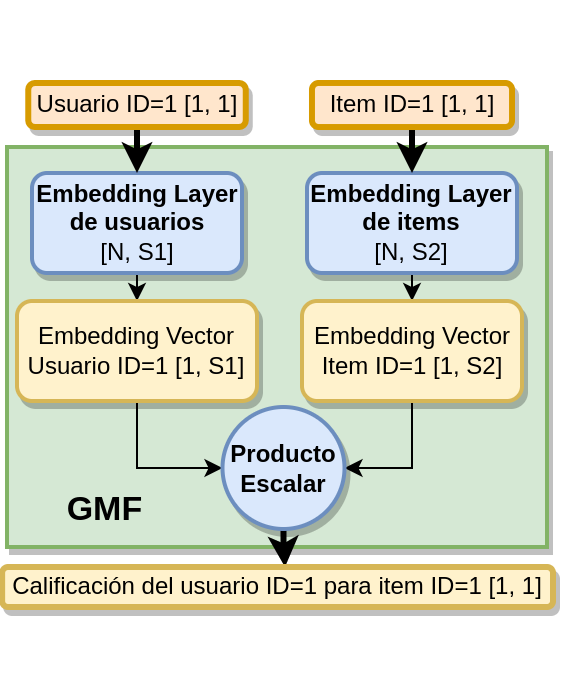
\includegraphics[width=6cm]{./images/GMF.png}
	\caption{
		Esquema de un modelo \textit{General Matrix Factorization (GMF)}.
	}
	\label{fig:GMFModel}
\end{figure}

\clearpage

En términos matemáticos este modelo realiza la siguiente operación, en cada
paso hacia adelante (\textit{forward-pass}):

\begin{equation}
	\tilde{r}_{u, i} = V_u . V_i^{T}
\end{equation}
\begin{description}
	\item[Donde:]
\end{description}
\begin{itemize}
	\item $V_u$ es el vector \textit{embedding} correspondiente al usuario $u$.
	\item $V_i^{T}$ el vector \textit{embedding} correspondiente al ítem $i$.
	\item $ \tilde{r}_{u, i}$ es la predicción de la calificación realizada por el usuario $u$ al ítem $i$ (valor escalar).
\end{itemize}

En términos matriciales podemos verlo de la siguiente manera:

\begin{equation}
	\tilde{R} = U.I
\end{equation}
\begin{description}
	\item[Donde:]
\end{description}
\begin{itemize}
	\item $U\in\mathbb{R}^{u \times f}$ es la matriz de vectores \textit{embedding} de usuarios, la cuál tiene tantas filas $u$ como usuarios y es la dimensión del número de columnas (también llamada factor latente) corresponde al tamaño seleccionado para los vectores \textit{embedding}.
	\item $I\in\mathbb{R}^{f\times items}$ es la matriz de vectores \textit{embeddings} de ítems, la cual tiene tantas filas como factores latente en los vectores \textit{embedding}, y tantas columnas como ítems se tenga.
	\item $\tilde{R}\in\mathbb{R}^{usuarios \times items}$ es la matriz de calificaciones, donde cada fila corresponde a un usuario y columna a un ítem.
\end{itemize}

El tamaño de la dimensión de factores latentes como ya se vio anteriormente en
el apartado \textit{One-Hot vs. Embeddings} es un hiper-parámetro mas a
ajustar. Se ha demostrado~\cite{embeddingsizedem} que realizar factorización de
matrices con un factor latente de tamaño 1 es equivalente a un modelo de
recomendación por popularidad, es decir que recomienda los ítems mas populares
sin tener en cuenta la personalización de las recomendaciones. Luego, a medida
que vamos incrementando el tamaño del factor latente estar recomendaciones
serán cada ves mas personalizadas aumentando la calidad de las mismas. Cuando
el tamaño del factor latente es muy grande, el modelos comienza a sobre ajustar
(\textit{overfitting}) y por ende la calidad de las recomendaciones comentara a
empeorar. Para solucionar este se suelen agregar términos de regularización en
la función de error a minimizar:

\begin{equation}
	\underset{H, W}{\operatorname{arg\,min } }\, \|R - \tilde{R}\|_{\rm F} + \alpha\|H\| + \beta\|W\|
\end{equation}
\begin{description}
	\item[Donde:]
\end{description}
\begin{itemize}
	\item $\|.\|_{\rm F}$ se define como [[norma matricial]] mientras que las otras normas pueden ser matricial u otro tipo de normal dependiendo del sistema de recomendación.
\end{itemize}

\subsection{\textit{Biased General Matrix Factorization (B-GMF)}}

El modelo \textit{GMF} de \textit{Simon Funk}~\cite{afm, dlwkrs} realiza
recomendaciones de muy buena calidad, pero tiene una limitación: sólo utilizar
interacciones usuario-ítem que tengan que ver con valores numéricos referidos a
interacciones explicitas, como calificaciones. Los sistemas de recomendación
modernos deben explotar todas las interacciones posibles, tanto explícitas
(calificaciones numéricas) como implícitas (me gusta, compras, vistas,
favoritos, etc..). Para solucionar este nuevo problema, donde es necesario usar
cualquier tipo de interacción usuario-ítem (explicita o implícita), se agrega
un \textit{bias} o sesgo para los usuarios, y otro para los ítems.

A Continuación se puede aprecia el diagrama del modelo, muy similar al diagrama
~\ref{fig:GMFModel}:

\begin{figure}[h!]
	\centering
	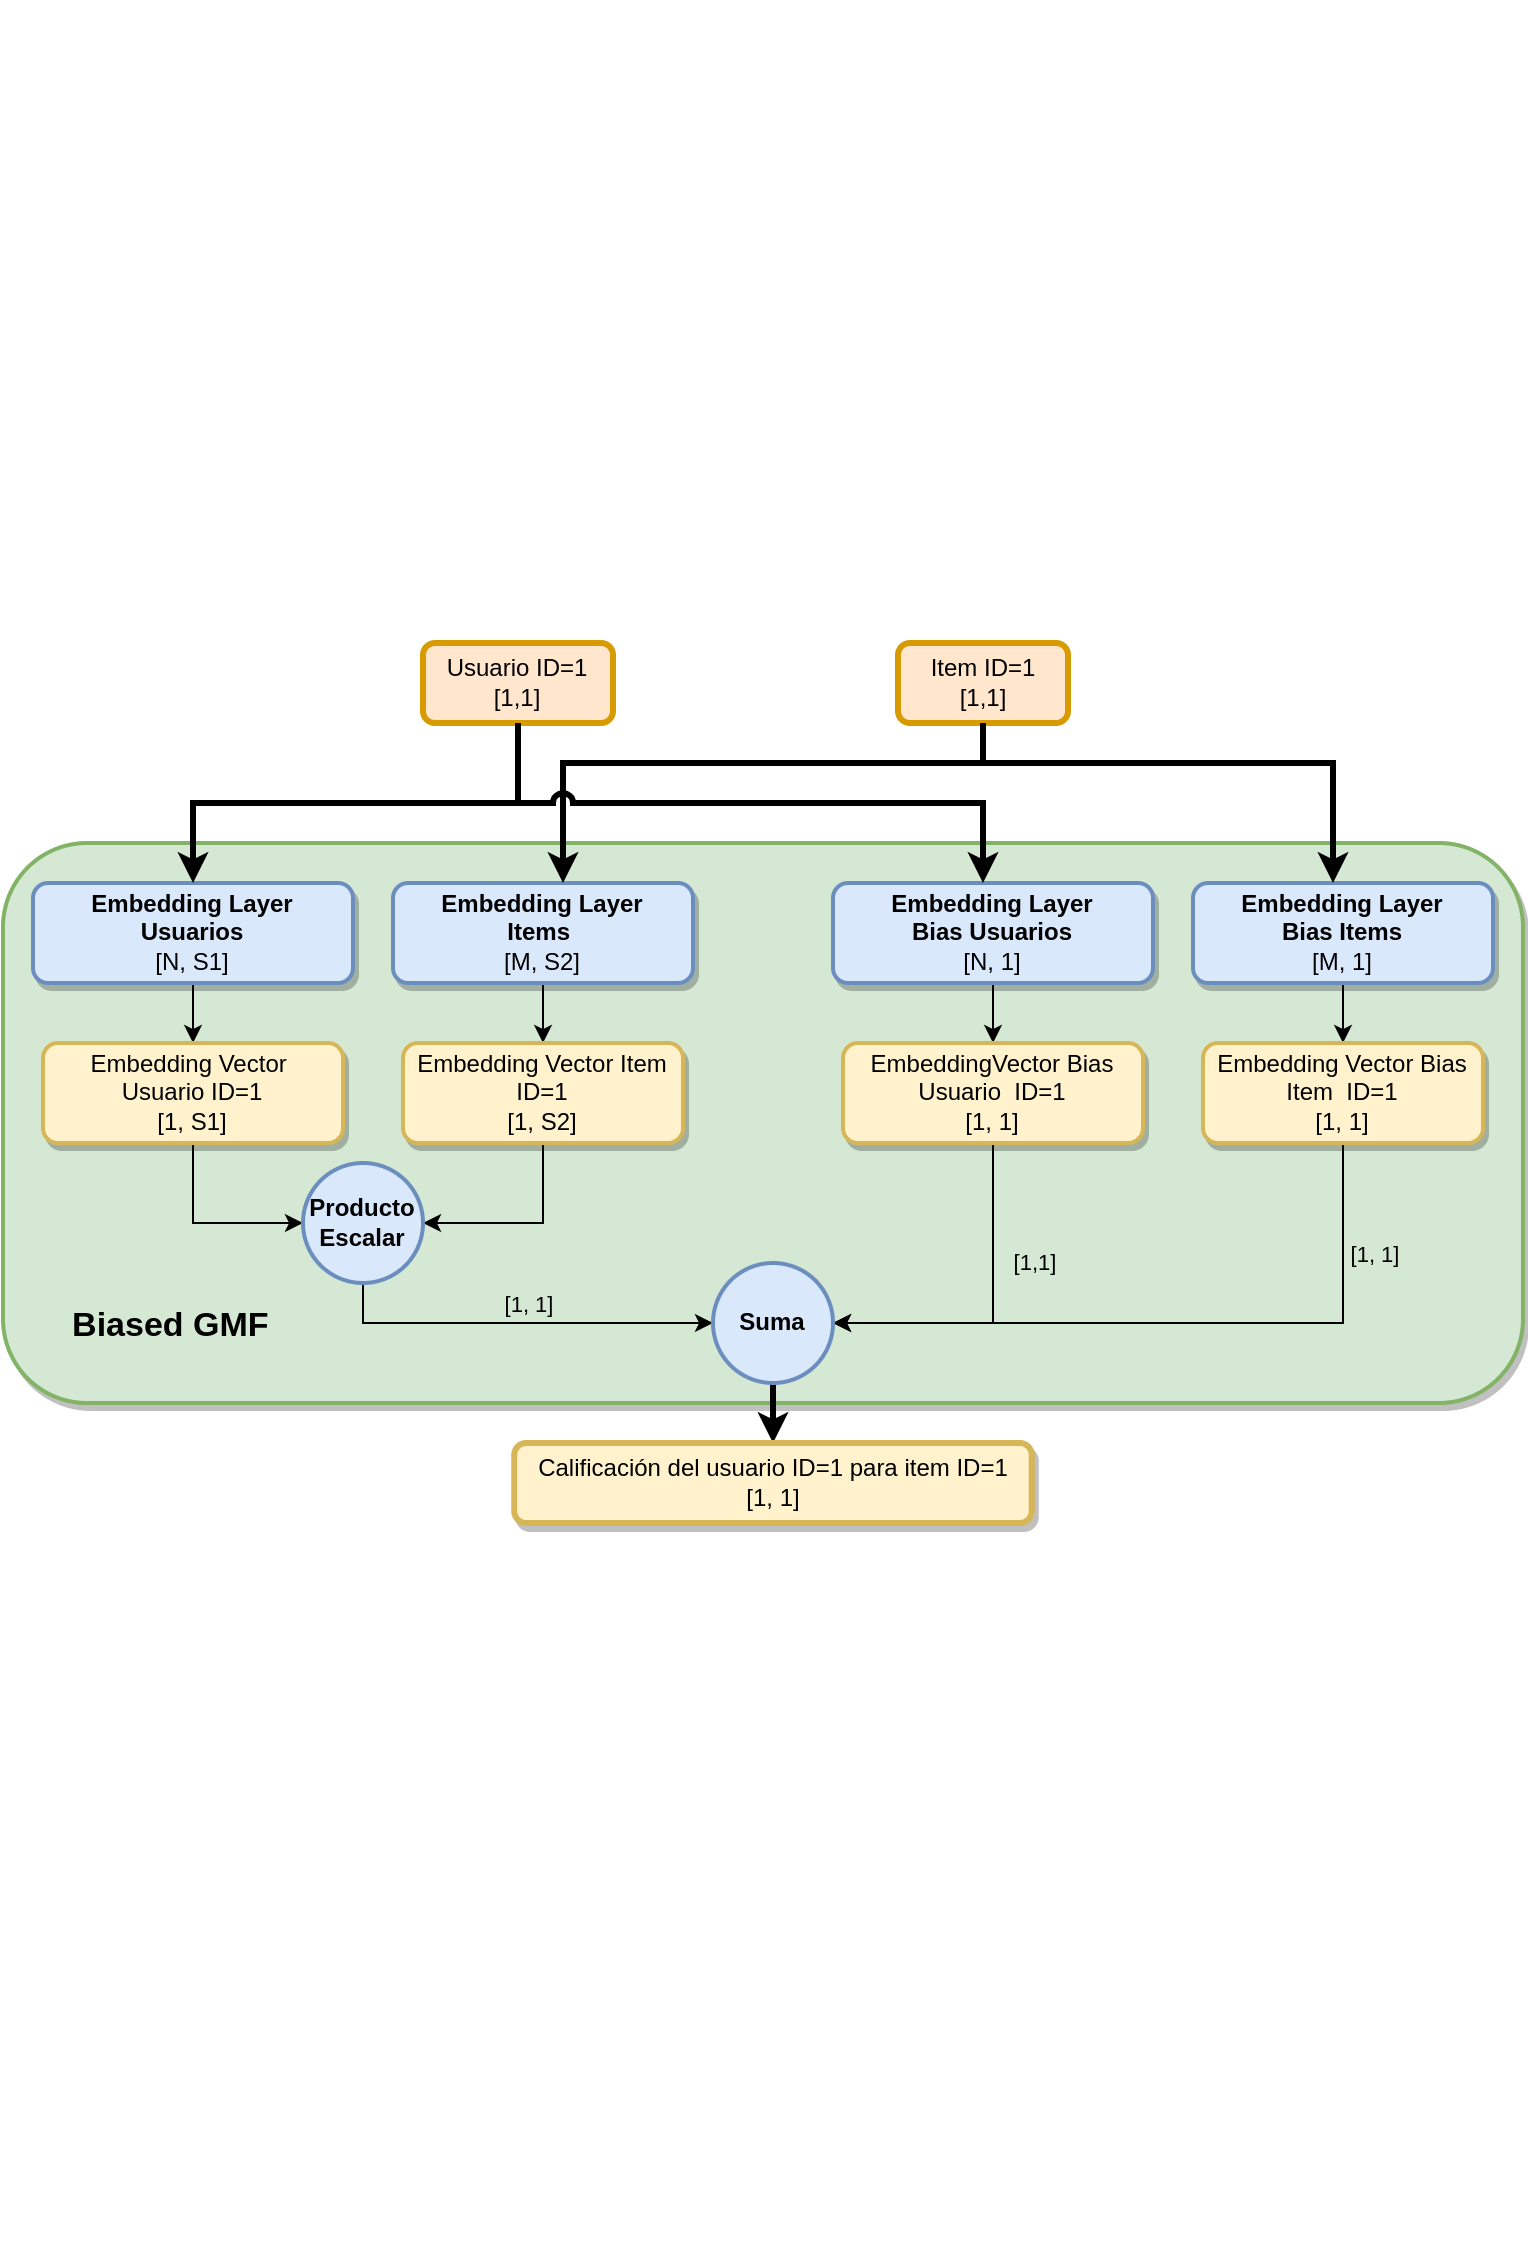
\includegraphics[width=11cm]{./images/Biased-GMF.png}
	\caption{
		Esquema de un modelo \textit{Biased General Matrix Factorization (B-GMF)}. A diferencia del modelo \textit{GMF}, este suma a la salida un \textit{bias} por cada variable de entrada.
	}
	\label{fig:BiasedGMFModel}
\end{figure}

En este caso se agregan dos nuevas \textit{Embedding Layers}, las cuales
representa a los sesgos de usuarios e ítems respectivamente. El tamaño de los
factores latentes o vectores \textit{embedding} correspondiente a cada
\textit{bias} es 1, es decir son valores escalares. Finalmente, luego de
calcular el producto escalar se suman los factores latentes resultado de ambas
\textit{Embedding Layers} correspondiente a los biases.

\clearpage

\subsection{\textit{Neural Network Matrix Factorization (NN-MF)}}

Con los enfoques anteriormente vistos (\textit{GFM} y \textit{Biased GFM}),
dada dos matrices de baja dimensionalidad se realiza un producto escalar y se
suman sesgos dependiendo de caso para calcular o inferir la calificación del
usuario para un ítem dado. Estos modelos, como ya se explico anteriormente,
aprender los pesos o parámetros de los vectores \textit{embeddings} en el
proceso se entrenamiento.

El enfoque de {\textit{NN-MF}}~\cite{nnfm}~\cite{ncf} es levemente distinto. En
este caso se reemplaza el producto interno, el cual podemos pensarlo como
conocimiento a priori del problema, por otra función desconocida, que sera la
que aprenderá el modelo a partir de las observaciones suministradas en el
entrenamiento. En particular, se remplaza el producto escalar sumado a los
sesgos, por una red neuronal multi capa de capas densas o \textit{fully
	connected}. De esta forma, el modelo no solo aprender los parámetros de los
vectores \textit{embedding}, sino también los pesos de la red multi capa. En
definitiva el modelo aprende cual es la mejor función para predecir las
calificaciones del usuario.

El uso de redes neuronales presenta una ventaja significativa: la posibilidad
de utilizar múltiples variables como entrada, no limitándose únicamente a las
variables categóricas usuario e ítem. Es precisamente en esta característica
donde radica su mayor potencial. No obstante, es importante mencionar que este
modelo muestra una ligera disminución en la precisión de sus predicciones en
comparación con modelos anteriores.

A continuación podemos ver un esquema del modelo, muy similar a \textit{GFM}
como ya se dijo, con la diferencia que tenemos una red multi capa en vez de un
producto escalar.

\begin{figure}[h!]
	\centering
	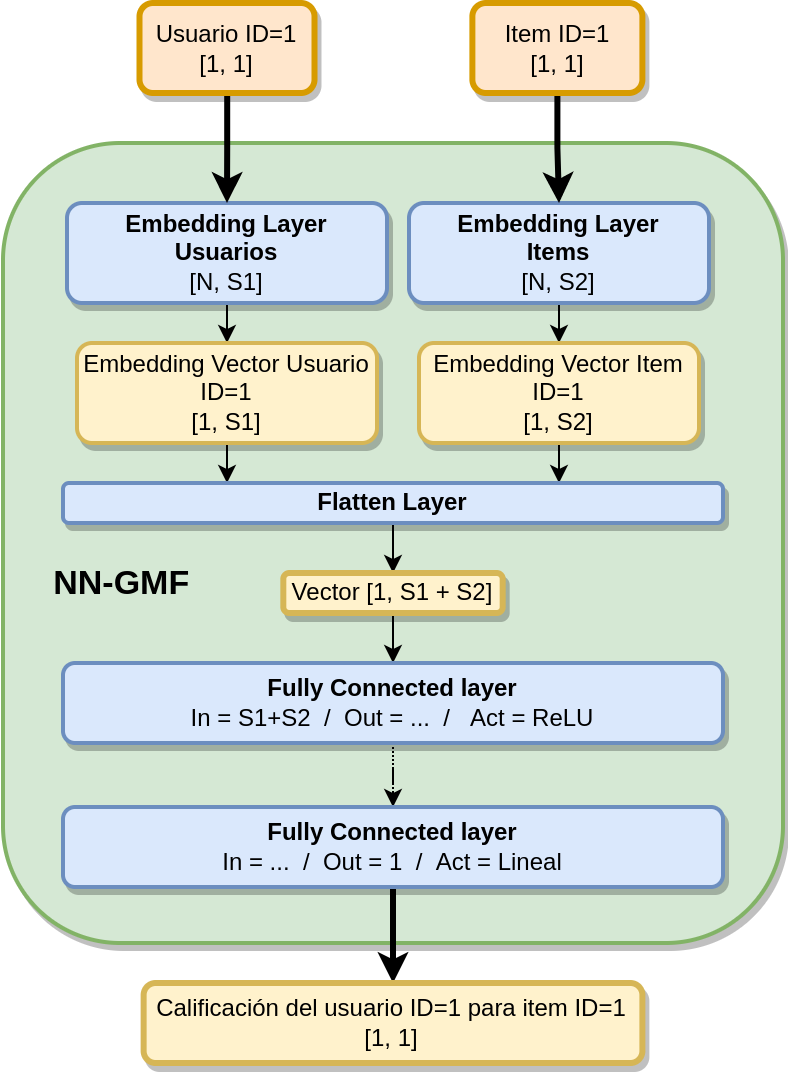
\includegraphics[width=6cm]{./images/NN-MF.png}

	\caption{
		Esquema de un modelo \textit{Neural Network Matrix Factorization (NN-MF)}.
	}
	\label{fig:NNMFModel}
\end{figure}

Para comenzar, el modelo tiene como entradas independientes los identificadores
de usuarios e ítems. Cada capa (\textit{Embedding Layer}) genera el
correspondiente vector \textit{embedding} asociado a estos identificadores. A
continuación, el bloque \textit{Flatter} toma ambos vectores y produce uno
nuevo mediante su concatenación. Este vector resultante se convierte en la
entrada de una red multi-capa.

Es importante destacar que la red multi-capa tendrá tantas entradas como
dimensiones posea este nuevo vector combinado. La cantidad de capas y el número
de neuronas por capa son hiper-parámetros que se ajustarán durante el proceso
de optimización. Por esta razón, no se especifica un número fijo de capas.

Cada capa, excepto la última, utiliza la función de activación \textit{ReLU},
mientras que la capa final emplea una activación \textit{Lineal}, similar a una
regresión lineal. Esto se debe a que el objetivo es predecir las
calificaciones, las cuales tienen un rango de valores reales entre $0.5$ y $5$.
Es importante señalar que se está considerando utilizar una activación
\textit{Softmax} en lugar de una activación \textit{Lineal} en la última capa,
lo que permitiría abordar el problema como uno de clasificación.

\clearpage

NOTA: La corrección de ortografía y semánticas llego hasta Aquí.

\subsection{\textit{Factorization Machines (FM)}}

Antes de introducir el modelo \textit{Deep Factorization Machine} se comenzara
explicando uno de sus componentes mas importantes: las máquinas de
factorización~\cite{didlfm, zhangdive}.

Las Maquinas de Factorización propuestas por \textit{Steffen Rendle} en 2010
~\cite{fm}, son algoritmos supervisados que se puede utilizar para tareas de
clasificación, regresión y tareas de ranking como sucede en el ámbito de los
sistemas de recomendación. Rápidamente se convivieron en un método popular para
hacer predicciones y recomendaciones. La \textit{Máquina de factorización} es
una generalización de un modelo lineal y un model de factorización de matrices,
mas aun, recuerdan mucho a un \textit{Maquina de soporte vectorial(SVM)} que
utiliza un kernel polinomial.

F Formalmente, si tenemos:

\begin{itemize}
	\item $x\in\mathbb{R}^{d}$ es un vector de features donde cada una de sus componentes representa a una variable del \textit{dataset}, siendo $d$ la cantidad de variables de \textit{dataset¨} (excluyendo la columna de labels). En nuestro caso $x\in\mathbb{R}^{2}$ ya que tenemos dos variables, usuarios e ítems.
	\item $y\in\mathbb{R}$ es la variable target a predecir. Dado el dominio del \textit{dataset} seleccionado, seria la calificación del usuario.
\end{itemize}

podemos definir el modelo para una \textit{máquina de factorización} de grado
dos de ls siguiente forma:

\begin{equation}
	\hat{y}(x) = \mathbf{w}_0 + \sum_{i=1}^d \mathbf{w}_i x_i + \sum_{i=1}^d\sum_{j=i+1}^d \langle\mathbf{v}_i, \mathbf{v}_j\rangle x_i x_j
\end{equation}
\begin{description}
	\item[Donde:]
\end{description}
\begin{itemize}
	\item $\mathbf{w}_0 \in \mathbb{R}$ es el bias global.
	\item $\mathbf{w} \in \mathbb{R}^d$ es el peso asociado a la variable $i^\mathrm{th}$.
	\item $\mathbf{V} \in \mathbb{R}^{d\times k}$ representa a un vector \textit{embedding} asociado al la variable $i^\mathrm{th}$.
	\item $\mathbf{v}_i$ representa a la $i^\mathrm{th}$ fila de la matriz $\mathbf{V}$.
	\item $k$ es la dimensionalidad del factor latente o tamaño de lso vectores \textit{embedding}.
	\item $\langle\cdot, \cdot \rangle$ es el producto interno de dos vectores.
	\item $\langle \mathbf{v}_i, \mathbf{v}_j \rangle$ modelos la interacción entre $i^\mathrm{th}$ y $j^\mathrm{th}$ variable.
\end{itemize}

De esta forma los dos primeros términos corresponden al modelo de regresión
lineal y el último término es una extensión del modelo de factorización
matricial. Si la variable $i$ representa un ítem y la variable $j$ a un
usuario, el tercer término es el producto escalar entre los vectores
\textit{embedding} de usuario $u$ y ítem $i$. Por otro lado, vale la pena
aclarar que este método también puede generalizar en órdenes superiores al
grado 2, sin embargo, la estabilidad numérica podría disminuí la generalización
del método.

Al aplicar un método de optimización con las máquinas de factorización, como
puede el método del gradiente descendente, se puede llegar fácilmente a una
complejidad del orden $\mathcal{O}(kd^2)$, ya que se deben calcular todas las
interacciones de a pares. Para resolver este problema de insuficiencia, podemos
reorganizar el tercer término del método, lo que podría reducir en gran medida
el costo de cálculo, lo que lleva a una complejidad de tiempo de orden lineal
$\mathcal{O}(kd)$. A continuación se describe los pasas para bajar el nivel de
complejidad del método:

\begin{equation}
	\begin{split}
		&=\sum_{i=1}^d \sum_{j=i+1}^d \langle\mathbf{v}_i, \mathbf{v}_j\rangle x_i x_j \\
		&= \frac{1}{2} \sum_{i=1}^d \sum_{j=1}^d\langle\mathbf{v}_i, \mathbf{v}_j\rangle x_i x_j - \frac{1}{2}\sum_{i=1}^d \langle\mathbf{v}_i, \mathbf{v}_i\rangle x_i x_i \\
		&= \frac{1}{2} \big (\sum_{i=1}^d \sum_{j=1}^d \sum_{l=1}^k\mathbf{v}_{i, l} \mathbf{v}_{j, l} x_i x_j - \sum_{i=1}^d \sum_{l=1}^k \mathbf{v}_{i, l} \mathbf{v}_{i, l} x_i x_i \big)\\
		&=  \frac{1}{2} \sum_{l=1}^k \big ((\sum_{i=1}^d \mathbf{v}_{i, l} x_i) (\sum_{j=1}^d \mathbf{v}_{j, l}x_j) - \sum_{i=1}^d \mathbf{v}_{i, l}^2 x_i^2 \big ) \\
		&= \frac{1}{2} \sum_{l=1}^k \big ((\sum_{i=1}^d \mathbf{v}_{i, l} x_i)^2 - \sum_{i=1}^d \mathbf{v}_{i, l}^2 x_i^2)
	\end{split}
\end{equation}

Con esta re-formulación de último termino, la complejidad del método se reduce
considerablemente. Además, para las variables ralas, solo se deben computar los
valores distintos de cero para que la complejidad general sea lineal.
Finalmente la expresión del método aplicada esta re-formulación queda como
sigue:

\begin{equation}
	\hat{y}(x) = \mathbf{w}_0 + \sum_{i=1}^d \mathbf{w}_i x_i + \frac{1}{2} \sum_{l=1}^k \big ((\sum_{i=1}^d \mathbf{v}_{i, l} x_i)^2 - \sum_{i=1}^d \mathbf{v}_{i, l}^2 x_i^2)
\end{equation}

\clearpage

\subsection{\textit{Deep Factorization Machine (DeepFM)}}

Hasta aquí, a grandes rasgos, todos los modelos expuestos tratan de captar el
comportamiento de las interacciones o correlación usuario-ítems, ya sean
implícitas o explicitas. A pesar de este gran progreso, los métodos expuestos
anteriormente (exceptuando las \textit{Máquinas de Factorización}) parecen
tener un fuerte sesgo al predecir las interacciones o correlaciones de bajo y
alto orden, requiriendo en algunos casos realizar ingeniería de features para
disminuir estos sesgos.

El modelo \textit{Deep Factorization Machine (DeepFM)}~\cite{dfmpaper, didldfm}
o Maquina de factorización basada en \textit{Deep Learning}, mejora el
aprendizaje de las interacciones o correlaciones de bajo y alto orden. Este
modelo combina \textit{Máquinas de Factorización} y \textit{Deep Learning} en
una nueva arquitectura de red neuronal la cual captura estas correlaciones. Por
otro lado, es una evolución del modelo \textit{Wide and
	Deep}~\cite{wideanddeeppaper} de \textit{Google}, el cual es un ensample de dos
modelos: uno lineal, que captura las interacciones o correlaciones de alto
orden y una MLP (\textit{Multi-Layer Perceptron}) la cual captura correlación
de mas bajo orden, o aquellas mas complejas.

A continuación de puede visualizar un diagrama de bloques de alto nivel de
modelos:

\begin{figure}[h!]
	\centering
	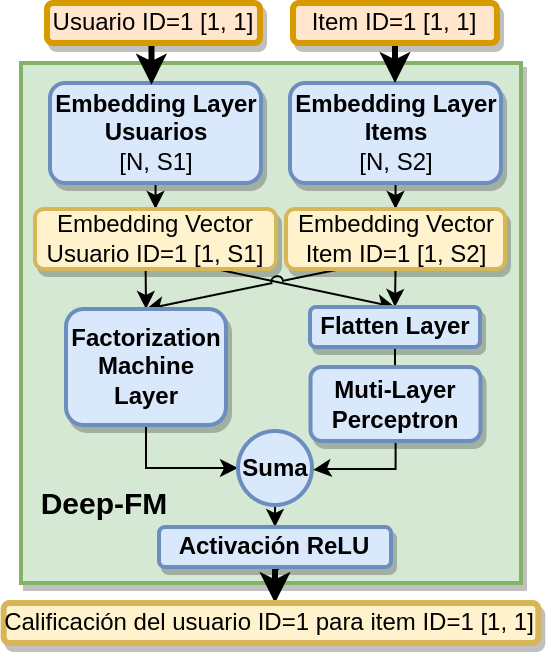
\includegraphics[width=6cm]{./images/Deep-MF.png}
	\caption{
		Esquema de un modelo \textit{Deep Factorization Machine (DeepFM)} o maquina de factorización basada en \textit{Deep Learning}.
	}
	\label{fig:DeepMFModel}
\end{figure}

Donde se puede apreciar que las entradas del modelo son las variables
categóricas correspondiente a usuarios e ítems, como en los modelos previamente
visto. Dado un id de usuario y ítem se resuelve sus correspondientes vectores
\textit{embedding}, los cuales se convierten en entradas para los siguientes
dos bloques. Uno de los bloques no es mas que una red neuronal multi capa con
capas densa o fully connected. Por el otro lado ambos vectores se toman como
entrada a la \textit{maquina de factorización}. Las salida de ambos bloques son
volares escalares los cuales se suman y se pasan por una activación
\textit{ReLU} ya que en nuestro caso las calificaciones son valores mayos a
cero.

\section{Métricas}

Para medir y comparar el grado de exactitude de los modelos seleccionados tanto
en el conjunto de validación como en truncamiento se seleccionado dos métricas:

\begin{itemize}
	\item \textit{Root Mean Square Error (RMSE)}: ES la raíz cuadrada del error cuadrático medio.
	\item \textit{Mean Average Precision at k (mAP@k)}: Es la media del promedio de la precision  para un tamaño K de observaciones.
\end{itemize}

\subsection{\textit{Root Mean Square Error (RMSE)}}

Dado que todos los modelo se evaluaron en este trabajo tiene como salida una
variable real (Calificación de los usuarios para un ítem), es posible utilizar
\textit{RMSE}, la cual es utilizada en problemas de regresión donde la salida
del modelo es una variable numérica real.

Si bien esta métrica no es la métrica por excelencia a usar en el ámbito de
sistemas de recomendación, ayuda a comprender cuales el grado de ajuste de los
modelos y pue servir como una métrica complementara al momento de evaluar los
mismos.

\begin{description}
	\item[Definición:]
\end{description}
\begin{equation}
	\operatorname{RMSE}=\sqrt{  \frac{1}{N} \sum_{i=1}^N (y_i - \hat y_i)^2}
\end{equation}
\begin{description}
	\item[Donde:]
\end{description}
\begin{itemize}
	\item $y_i$ es el true value o verdad de campo de la observación.
	\item $\hat y_i$ es la predicción realizada por el modelo predictor.
	\item $N$ es el numero de observaciones sobre las que se realizo la predicción del modelo.
\end{itemize}

\subsection{\textit{Mean Average Precision at k (mAP@k)}}

\textit{Mean Average Precision at k (mAP@k)} o media del promedió de la precision para K observaciones, es una de las métricas mas usada para evaluar sistemas de recomendación~\cite{map_at_k_1, map_at_k_2, map_at_k_3}.

Si pensamos a nivel de aplicación de un sistemas de recomendación pedimos ver
entras y salidas donde:

\begin{itemize}
	\item Entradas: Como entradas tenemos el identificador del usuario al cual queremos
	      presentarle recomendaciones y otro parámetro opcional que podría ser el
	      identificador de un ítem. ¿Por que opcional? Bueno, en general si no
	      especificamos un id de ítem, es posible encontrar cuales son los ítems de mayor
	      preferencia para el usuario y luego recomendar nuevos ítems en base a este ítem
	      inicial. Por otro lado, si ya se cuenta con un id de ítem, se puede recomendar
	      ítems similares en este. Este ultimo caso es muy común cuando un usuario navega
	      al detalle de un producto en un e-commerce. En esta instancia, ya se conoce el
	      id del usuario y id de ítem. Finalmente se recomiendan ítems similares al ítem
	      visualizado.
	\item Salidas: Es una lista de ítems recomendados similares a otro ítem (Entrada del
	      modelo) ordenados descendente-mente por la calificación predicha por el modelo
	      para el usuario en cuestión (Entrada del modelo).
\end{itemize}

De esta forma, encontrar en las primeras posiciones de la lista, aquellos ítems
con mayor calificación predicha, es un indicador de que el modelo es preciso al
momento de recomendar. En palabras mas simples, se desea que los primeros ítems
de la lista de recomendaciones sean de mayor agrado para el usuario.\newline

¿Finalmente, como funciona esta métricas? La métrica \textit{mAP\makeatletter@k} funciona de la siguiente forma: \newline

Supongamos que tenemos un usuario y una lista K de ítems a recomendar. En base
a estas entradas el modelo de recomendación predice las calificaciones de cada
ítem para el usuario dado. Luego, podemos ordenar la lista de ítems
descendente-mente de acuerdo a las calificaciones predichas por el modelo.

Teniendo esta lista, se puede calcular el promedio de la predicción
\textit{mAP\makeatletter@k} sobre los K ítems de la lista.

Esta métrica es utilizada en problemas de clasificación pero también se puede
utilizar en problemas donde el modelo produce una salida numérica como en este
caso. Los niveles o clases a utilizar dependen mucho de que se quiera evaluar.
Supongamos, en este caso particular, que queremos medir con que precisión
aparecen las puntuaciones entre 4 y 5 en las primera posiciones de la lista.
Para este fin se utilizara la métricas \textit{mAP\makeatletter@k}.

\begin{description}
	\item[Promedio de la precisión sobre una lista de K elementos
	\textit{AP\makeatletter@k}:]
\end{description}
\begin{equation}
	\begin{split}
		& \operatorname{AP\makeatletter@k}=\frac{1}{N(k)} \sum_{i=1}^k \frac{ TP(i)}{i}, \\
		& \\
		& \operatorname{N(k)} = min(k, TP_{total}) \\
	\end{split}
\end{equation}
\begin{description}
	\item[Donde:]
\end{description}
\begin{itemize}
	\item $i$ es la posición del ítem $i^\mathrm{th}$ en la lista de $k$ elementos. $i$  toma valores entre $1$ y $k$.
	\item $TP_i$ es 1 si la precision y el valor verdadero concuerdan.
	\item $N(k)$ es el mínimo entre el tamaño de la lista y la cantidad de $TP_{total}$ encontrados en esa lista.
\end{itemize}

Por ejemplo, si se quiere saber con que precisión aparecen ítems con
calificaciones entre 4 y 5 puntos en las primeras posiciones de la lista:

\begin{itemize}
	\item Si $TP_i$ es igual a $1$, entonces la calificación en la posición
	      $i^\mathrm{th}$ se encuentra entre los 4 y 5 punto.
	\item Si $TP_i$ es igual a $0$, entonces la calificación en la posición
	      $i^\mathrm{th}$ NO se encuentra entre los 4 y 5 punto.
\end{itemize}

De esta forma, se esta transformando la salida del modelo en una lista de
valores binarios. Donde la clase 1 indica que se cumple con la condición
esperada y la clase 0 lo contrario.

Luego se realiza el calculo de \textit{AP\makeatletter@k} para cada usuario del
\textit{dataset} de validación y finalmente se calcula la media:

\begin{description}
	\item[Media del promedio de la precisión sobre una lista de K elementos
	\textit{mAP\makeatletter@k}:]
\end{description}
\begin{equation}
	\operatorname{mAP\makeatletter@k}=\frac{1}{N} \sum_{i=1}^N AP\makeatletter@k_i
\end{equation}

De esta forma, la métrica \textit{mAP\makeatletter@k} da una noción del grado
de precisión en que aparecen ítems con mayor puntuación en las primeras
posiciones de una lista de tamaño $k$. Cabe aclarar, que la condición
\textit{ítems con mayor puntuación} es arbitraria, ua que al ser una condición,
podríamos intercambiarla por cualquier otro criterio. Por ejemplo, ítem con las
peores puntuaciones (entre 1 y 2 puntos), ítem con puntuaciones medias, ítems
con mas de 3 puntos, menos de 3 puntos, etc...

\chapter{Experimentos}

Para comparar todos los modelos implementados, se utilizo el mismo
\textit{dataset}, tomando una muestra con el tamaño suficiente para obtener
buenos resultados, evitando el sobre ajuste(\textit{overfitting}) con aquellos
modelos que tienden a sobre ajustar mas. Por otro lado, se realizo una
modificación al modelo \textit{KNN} para poder guardar sus resultados en una
memoria \textit{Cache}. De esta forma, no se repite la inferencia de las
predicciones al momento de seleccionar muestras del conjuntos de validación,
disminuyendo notablemente el tiempo de inferencia.

Por otro lado, cabe aclarar que dada la tendencia de los modelos a la
variabilidad o varianza de sus predicciones, se realizo N veces un muestreo
sobre el conjunto de validación para cada métrica utilizada. Luego, se gráfico
un histograma de la distribución de la métricas, y un boxplot para tener una
mejor idea de cual es su valor medio y la dispersion se puede esperar.

A continuación se describen los resultados de todos los modelos comparados
mediando las métricas \textit{AP\makeatletter@k} y \textit{RMSE}.

\section{\textit{K-Nearest-Neighbor (KNN)}}

\subsection{\textit{KNN Item Based}}

\begin{figure}[!htb]
	\centering
	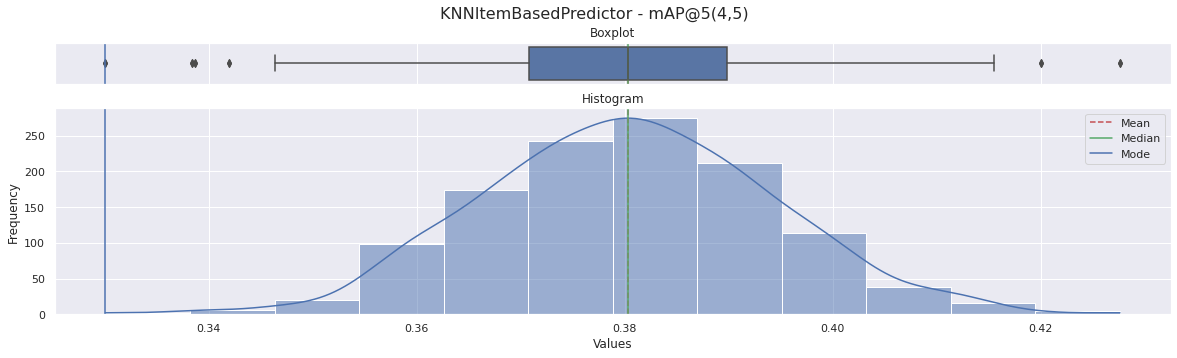
\includegraphics[width=15cm]{./images/metrics-knn-item-based-mapk.png}
	\caption{Esta gráfica describe un histograma del valor de la métrica \textit{mAP@5(4,5)} evaluado en el conjunto de observaciones de validación, luego de N procesos de entrenamiento del modelo \textit{KNN Item Based} sobre las observaciones de entrenamiento.}
\end{figure}

\clearpage

\begin{figure}[!htb]
	\centering
	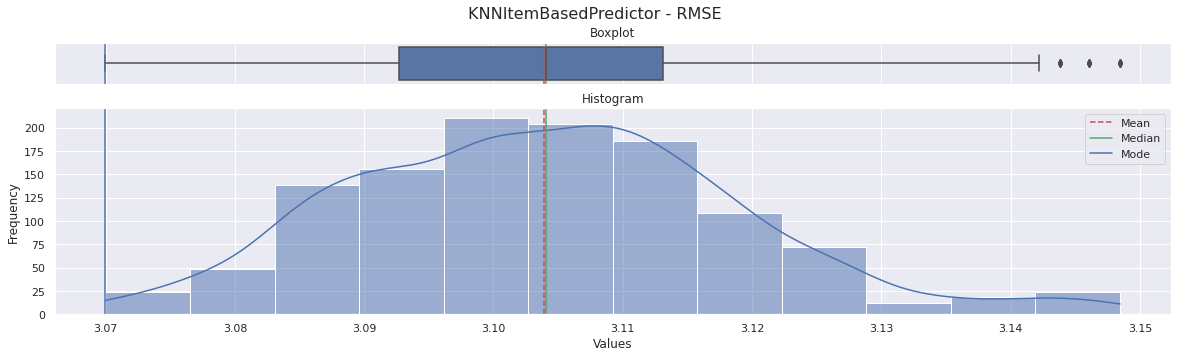
\includegraphics[width=15cm]{./images/metrics-knn-item-based-RMSE.png}
	\caption{Esta gráfica describe un histograma del valor de la métrica \textit{RMSE} evaluado en el conjunto de observaciones de validación, luego de N procesos de entrenamiento del modelo \textit{KNN Item Based} sobre las observaciones de entrenamiento.}
\end{figure}

\subsection{\textit{KNN User Based}}

\begin{figure}[!htb]
	\centering
	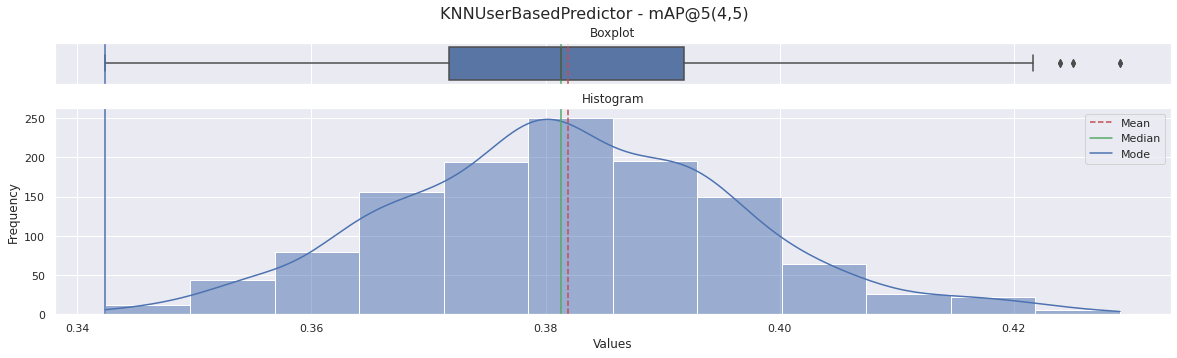
\includegraphics[width=15cm]{./images/metrics-knn-user-based-mapk.png}
	\caption{Esta gráfica describe un histograma del valor de la métrica \textit{mAP@5(4,5)} evaluado en el conjunto de observaciones de validación, luego de N procesos de entrenamiento del modelo \textit{KNN User Based} sobre las observaciones de entrenamiento.}
\end{figure}

\begin{figure}[!htb]
	\centering
	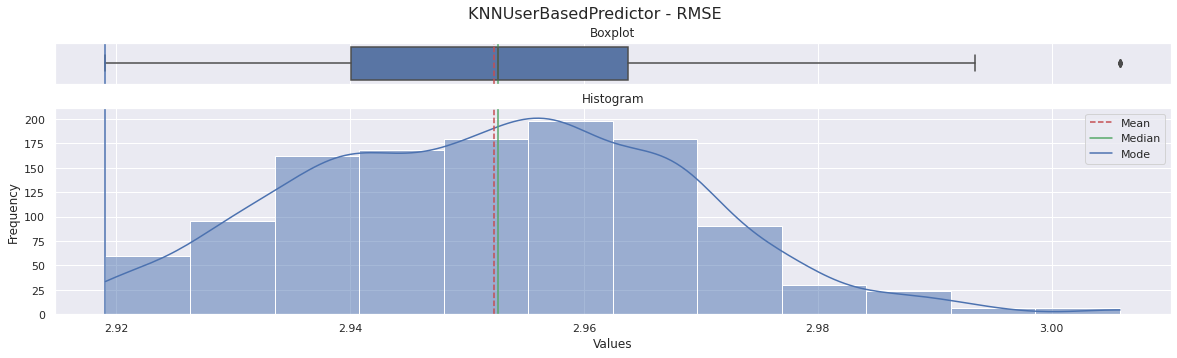
\includegraphics[width=15cm]{./images/metrics-knn-user-based-RMSE.png}
	\caption{Esta gráfica describe un histograma del valor de la métrica \textit{RMSE} evaluado en el conjunto de observaciones de validación, luego de N procesos de entrenamiento del modelo \textit{KNN User Based} sobre las observaciones de entrenamiento.}
\end{figure}

\clearpage

\subsection{\textit{KNN User Based Ensemble} y \textit{Item Based}}

\begin{figure}[!htb]
	\centering
	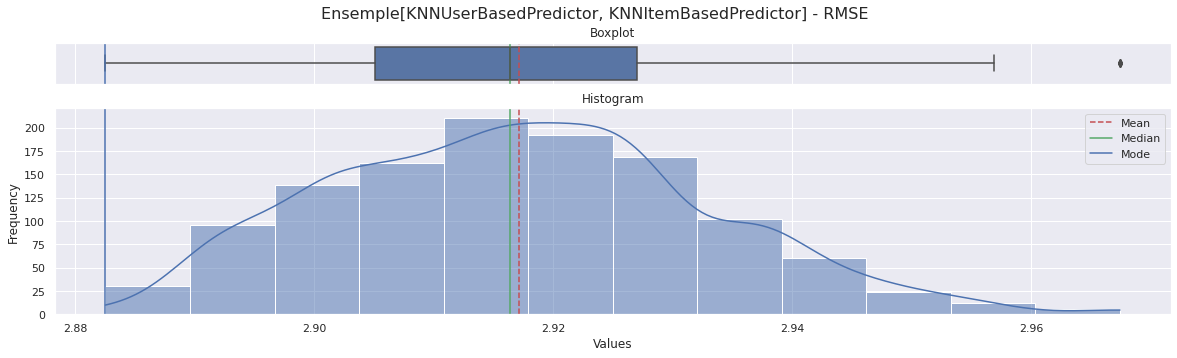
\includegraphics[width=15cm]{./images/metrics-knn-ensemple-RMSE.png}
	\caption{Esta gráfica describe un histograma del valor de la métrica \textit{RMSE} evaluado en el conjunto de observaciones de validación, luego de N procesos de entrenamiento del modelo \textit{KNN} sobre las observaciones de entrenamiento.}
\end{figure}

\begin{figure}[!htb]
	\centering
	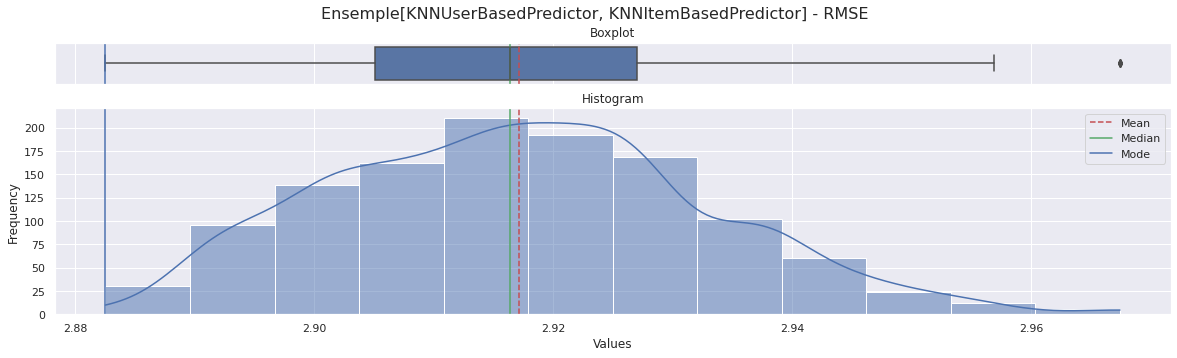
\includegraphics[width=15cm]{./images/metrics-knn-ensemple-RMSE.png}
	\caption{Esta gráfica describe un histograma del valor de la métrica \textit{RMSE} evaluado en el conjunto de observaciones de validación, luego de N procesos de entrenamiento del modelo \textit{KNN} sobre las observaciones de entrenamiento.}
\end{figure}

\clearpage
\section{\textit{General Matrix Factorization (GFM)}}

A continuación se puede apreciar las cursas de la $Loss$ (\textit{MSE}) para el
conjunto de validación y entrenamiento:

\begin{figure}[ht]
	\centering
	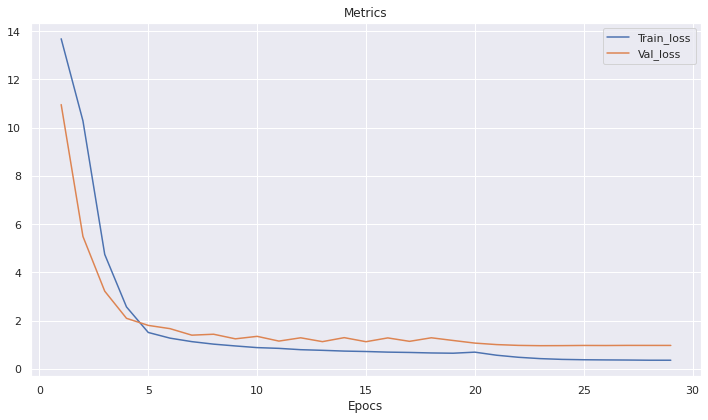
\includegraphics[width=13cm]{./images/metrics-GFM-train-val-loss.png}
	\caption{Esta gráfica describe el nivel de error sobre los conjuntos de observaciones de entrenamiento y validación durante el entrenamiento del modelo \textit{GFM}. Cada epoch o época indica una iteración de entrenamiento del modelo sobre el conjunto completo de entrenamiento.}
\end{figure}

Se puede apreciar que inicialmente el modelo tiene un error de valoración menor
al error de entrenamiento. Es posible que se deba a que una pocas primeras
observaciones de entrenamiento fueron suficientes para predecir con un error
menor el conjunto de validación. A media que se incrementa el numero de épocas
ya no es subiente y el modelo comienza a sobre ajusta hasta estabilizarse ambos
errores.

\clearpage

\begin{figure}[h!]
	\centering
	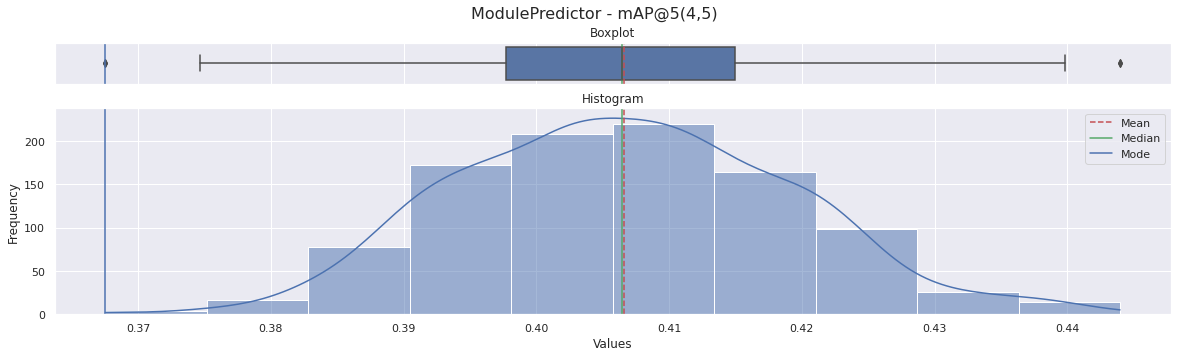
\includegraphics[width=15cm]{./images/metrics-GFM-mapk.png}
	\caption{Esta gráfica describe un histograma del valor de la métrica \textit{mAP@5(4,5)} evaluado en el conjunto de observaciones de validación, luego de N procesos de entrenamiento del modelo \textit{GFM} sobre las observaciones de entrenamiento.}
\end{figure}

Dado la tendencia de los modelos a la variabilidad o varianza de sus
predicciones se realizo un \textit{sampling} de cada métrica sobre el conjunto
de validación N veces para comprender cual es su valor medio y dispersión.

\begin{figure}[h!]
	\centering
	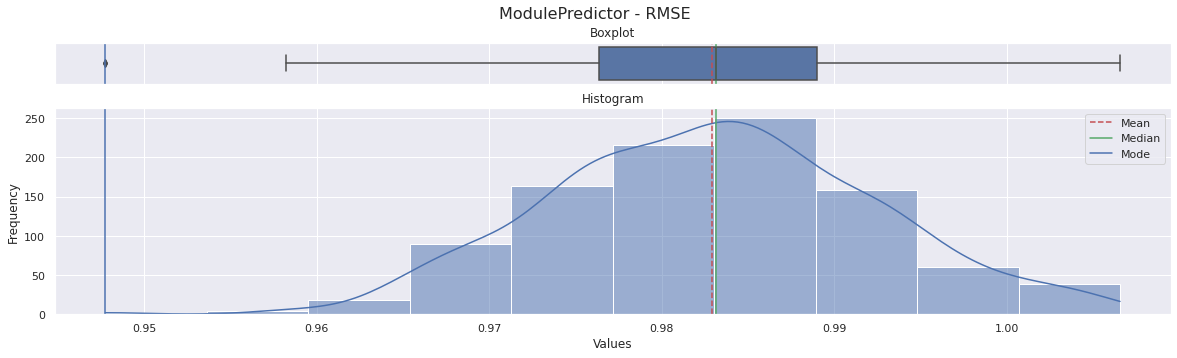
\includegraphics[width=15cm]{./images/metrics-GFM-RMSE.png}
	\caption{Esta gráfica describe un histograma del valor de la métrica \textit{RMSE} evaluado en el conjunto de observaciones de validación, luego de N procesos de entrenamiento del modelo \textit{GFM} sobre las observaciones de entrenamiento.}
\end{figure}

\clearpage
\section{\textit{Biased General Matrix Factorization (B-GFM)}}

\begin{figure}[h!]
	\centering
	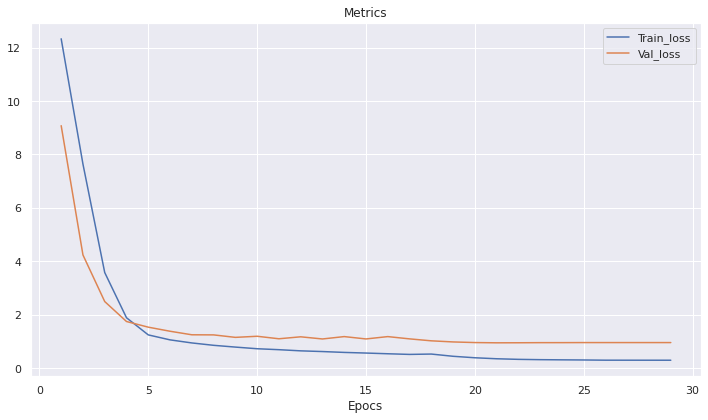
\includegraphics[width=13cm]{./images/metrics-BGFM-train-val-loss.png}
	\caption{Esta gráfica describe el nivel de error sobre los conjuntos de observaciones de entrenamiento y validación durante el entrenamiento del modelo \textit{B-GFM}. Cada epoch o época indica una iteración de entrenamiento del modelo sobre el conjunto completo de entrenamiento.}
\end{figure}

\begin{figure}[h!]
	\centering
	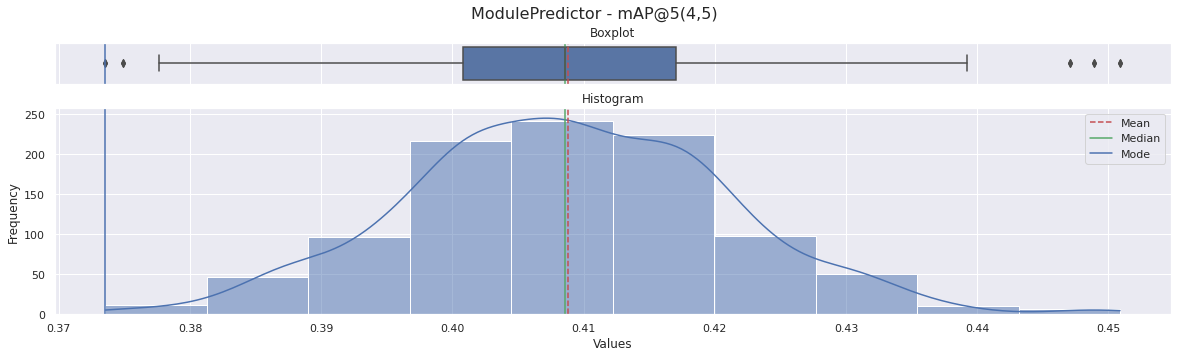
\includegraphics[width=15cm]{./images/metrics-BGFM-mapk.png}
	\caption{Esta gráfica describe un histograma del valor de la métrica \textit{mAP@5(4,5)} evaluado en el conjunto de observaciones de validación, luego de N procesos de entrenamiento del modelo \textit{B-GFM} sobre las observaciones de entrenamiento.}
\end{figure}

\clearpage

\begin{figure}[h!]
	\centering
	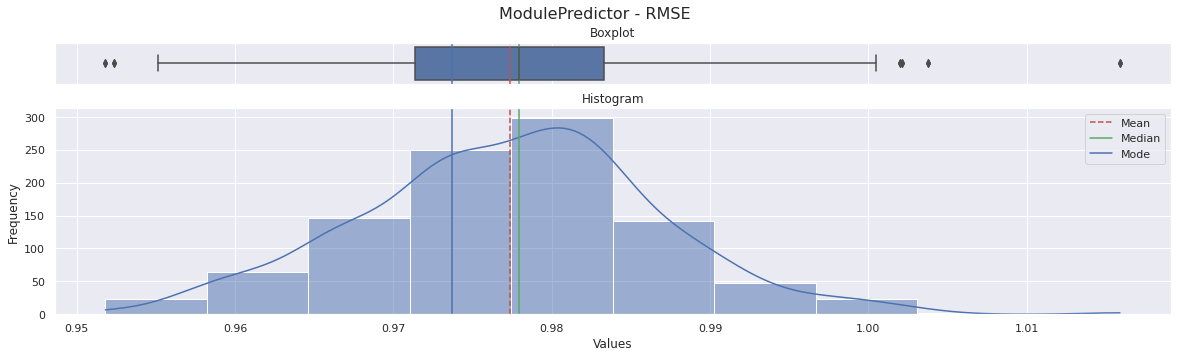
\includegraphics[width=15cm]{./images/metrics-BGFM-RMSE.png}
	\caption{Esta gráfica describe un histograma del valor de la métrica \textit{RMSE} evaluado en el conjunto de observaciones de validación, luego de N procesos de entrenamiento del modelo \textit{B-GFM} sobre las observaciones de entrenamiento.}
\end{figure}

\section{\textit{Neural Network Matrix Factorization (NN-FM)}}

\begin{figure}[h!]
	\centering
	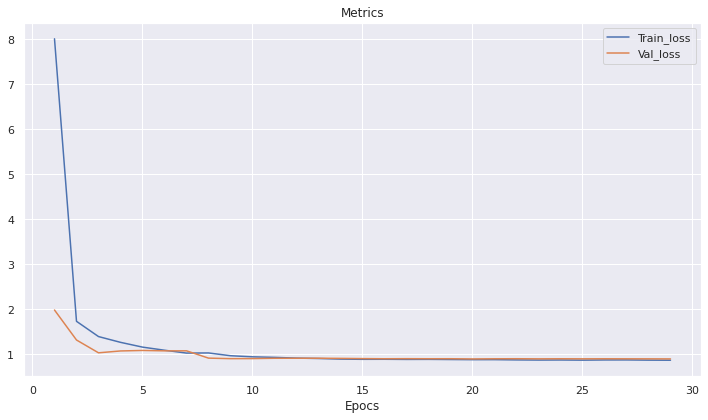
\includegraphics[width=13cm]{./images/metrics-NN-FM-train-val-loss.png}
	\caption{Esta gráfica describe el nivel de error sobre los conjuntos de observaciones de entrenamiento y validación durante el entrenamiento del modelo \textit{NN-FM}. Cada epoch o época indica una iteración de entrenamiento del modelo sobre el conjunto completo de entrenamiento.}
\end{figure}

\clearpage

\begin{figure}[h!]
	\centering
	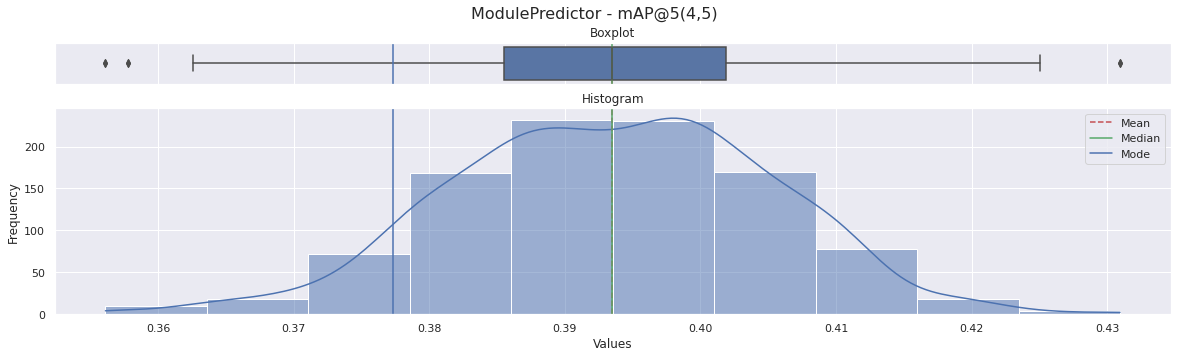
\includegraphics[width=15cm]{./images/metrics-NN-FM-mapk.png}
	\caption{Esta gráfica describe un histograma del valor de la métrica \textit{mAP@5(4,5)} evaluado en el conjunto de observaciones de validación, luego de N procesos de entrenamiento del modelo \textit{NN-FM} sobre las observaciones de entrenamiento.}
\end{figure}

\begin{figure}[h!]
	\centering
	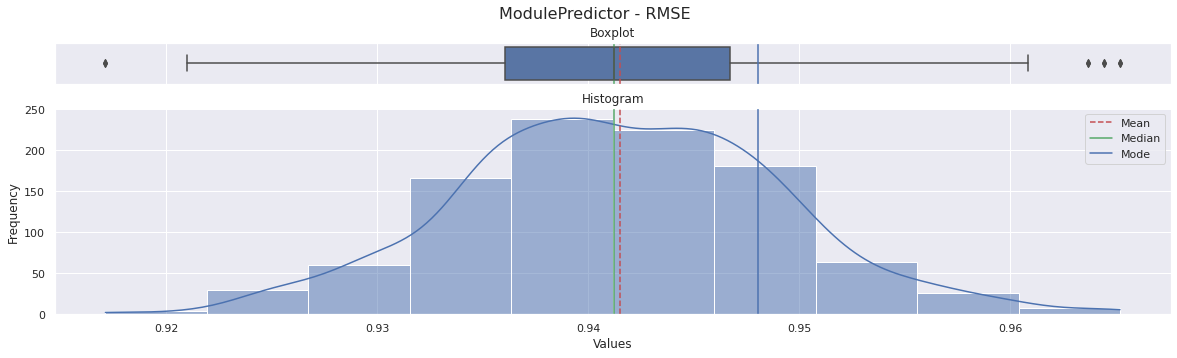
\includegraphics[width=15cm]{./images/metrics-NN-FM-RMSE.png}
	\caption{Esta gráfica describe un histograma del valor de la métrica \textit{RMSE} evaluado en el conjunto de observaciones de validación, luego de N procesos de entrenamiento del modelo \textit{NN-FM} sobre las observaciones de entrenamiento.}
\end{figure}

\clearpage

\section{\textit{Deep Factorization Machine (DeepFM)}}

\begin{figure}[h!]
	\centering
	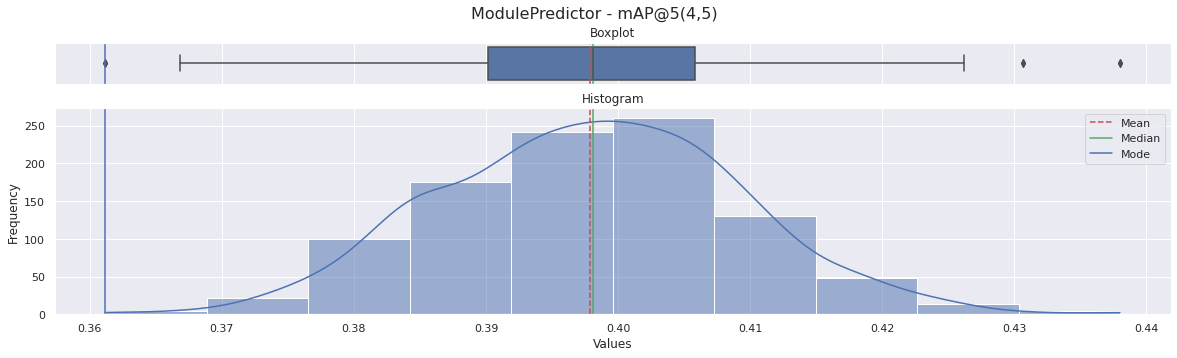
\includegraphics[width=15cm]{./images/metrics-DeepFM-mapk.png}
	\caption{Esta gráfica describe un histograma del valor de la métrica \textit{mAP@5(4,5)} evaluado en el conjunto de observaciones de validación, luego de N procesos de entrenamiento del modelo \textit{DeepFM} sobre las observaciones de entrenamiento.}
\end{figure}

\begin{figure}[h!]
	\centering
	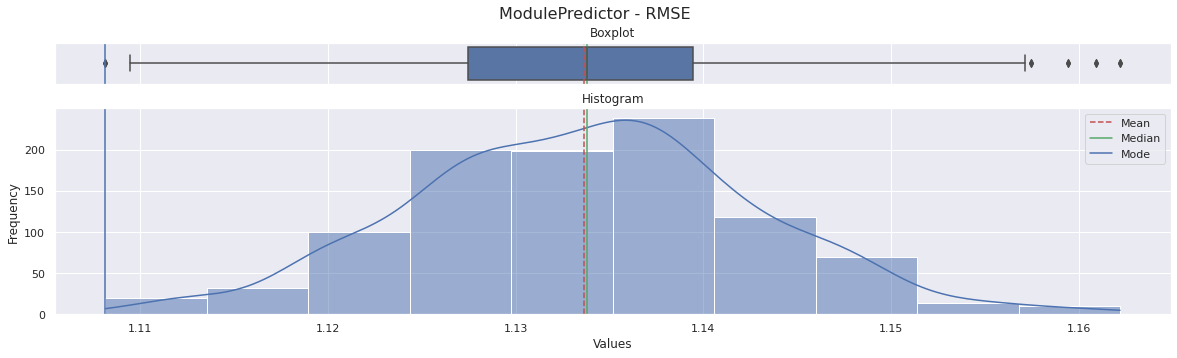
\includegraphics[width=15cm]{./images/metrics-DeepFM-RMSE.png}
	\caption{Esta gráfica describe un histograma del valor de la métrica \textit{RMSE} evaluado en el conjunto de observaciones de validación, luego de N procesos de entrenamiento del modelo \textit{DeepFM} sobre las observaciones de entrenamiento.}
\end{figure}

\chapter{Resultados}

En esta sección se llevará a cabo una comparación de todos los modelos
previamente expuestos. Para realizar esta comparación, se emplearán las
métricas presentadas en secciones anteriores. A modo de resumen, las métricas
consideradas fueron las siguientes:

\begin{itemize}
	\item \textit{Mean Average Precision at k (mAP@k)}: Esta métrica representa el promedio de la precisión al calificar
	      los primeros K ítems de una lista de recomendaciones para un usuario específico.
	      Para obtener más detalles, se puede consultar la sección de referencia sobre \textit{mAP@k} (consultar la \autoref{sec:map_ref}).
	\item \textit{Root Mean Square Error (RMSE)}: Esta métrica corresponde a la raíz cuadrada del error cuadrático
	      medio entre la calificación real de un ítem, proporcionada por un usuario, y la calificación predicha. Para obtener más información,
	      se puede consultar la sección de referencia sobre \textit{RMSE} (consultar la \autoref{sec:rmse_ref}).
\end{itemize}

Para calcular estas métricas, se realizo un muestreo para determinar su
distribución y, de esta forma, definir cada métrica en términos de su mediana,
media y desvío.

El uso de la media y el desvío estándar permite obtener el valor promedio de
las métricas y evaluar su grado de dispersión en los datos obtenidos. La media
nos proporciona una idea del valor típico de las métricas en el conjunto de
prueba, mientras que el desvío estándar nos indica qué tan dispersos están los
valores las metricas en relación con la media.

Además, se presenta la mediana como otra medida estadística relevante. A
diferencia de la media, la mediana no se ve afectada por valores atípicos o
extremos en el conjunto de datos, lo que la convierte en una medida más robusta
para describir la ubicación central de las métricas.

A continuación, se presenta la comparación de todos los modelos expuestos
utilizando el promedio de la precisión para el rango de calificaciones entre 4
y 5 puntos, considerando una lista de 5 items recomendados, que se denota como
\textit{AP@5(4,5)}:

\begin{table}[!htb]
	\centering
	\footnotesize
	\begin{tabular}{lrrr}
		\hline
		Modelo                                & Mediana  & Media    & Desvío   \\
		\hline
		\textit{B-GMF}                        & 0.408563 & 0.408787 & 0.012190 \\
		\textit{GMF}                          & 0.406422 & 0.406646 & 0.012513 \\
		\textit{DeepFM}                       & 0.398100 & 0.397895 & 0.011369 \\
		\textit{NN-MF}                        & 0.393499 & 0.393447 & 0.011711 \\
		\textit{KNN User-Item Based Ensemble} & 0.384570 & 0.384819 & 0.015066 \\
		\textit{KNN User Based}               & 0.381297 & 0.381943 & 0.014709 \\
		\textit{KNN Item Based}               & 0.380284 & 0.380327 & 0.014056 \\
		\hline
	\end{tabular}
	\caption{
		Mediana, media y desvío correspondientes a la distribución de
		\textit{AP\makeatletter@5(4,5)} muestreada para cada modelo. Las filas se encuentran ordenadas descendente-mente por la media.
	}
	\label{table:ap_at_k}
\end{table}

En la tabla~\ref{table:ap_at_k}, se puede observar inicialmente que el modelo
\textit{Biased-GMF} muestra los mejores resultados en términos de la métrica de
evaluación \textit{AP@5(4,5)}. Por otro lado, los modelos \textit{NN-MF} y
\textit{Deep-FM} exhiben el menor sesgo, pero aún así, tienen una precisión
inferior al modelo \textit{Biased-GMF}. Esto podría indicar un mayor grado de
sobreajuste en estos modelos. Por lo tanto, sería recomendable reentrenar ambos
modelos con un aumento en el valor del parámetro \textit{dropout} para mejorar
la regularización y, posteriormente, comparar nuevamente sus resultados con el
modelo \textit{Biased-GMF} para validar si su precisión mejora.

En cuanto a la familia de modelos \textit{KNN}, se observa que presenta el
mayor sesgo. Sin embargo, a pesar de esto, se puede notar que la diferencia en
la precisión, en comparación con los demás modelos, es bastante baja, siendo
menos del 2%.

En resumen, los resultados muestran que el modelo \textit{Biased-GMF} sobresale
en precisión según la métrica \textit{AP@5(4,5)}. Los modelos \textit{NN-MF} y
\textit{Deep-FM}, aunque tienen menos sesgo, deben ser reentrenados con un
mayor valor de \textit{dropout} para potencialmente mejorar su precisión. Por
otro lado, la familia de modelos \textit{KNN}, a pesar de presentar un sesgo
más alto, aún logra una precisión cercana a los demás modelos en comparación.
\clearpage

A continuación, se presenta la comparación de todos los modelos expuestos
utilizando utilizando la raíz cuadrada del error cuadrático medio
(\textit{RMSE}):

\begin{table}[!htb]
	\centering
	\footnotesize
	\begin{tabular}{lrrr}
		\hline
		Modelo                                & Mediana  & Media    & Desvío   \\
		\hline
		\textit{NN-MF}                        & 0.941213 & 0.941493 & 0.007620 \\
		\textit{B-GMF}                        & 0.977914 & 0.977382 & 0.009387 \\
		\textit{GMF}                          & 0.983141 & 0.982894 & 0.009419 \\
		\textit{DeepFM}                       & 1.133796 & 1.133637 & 0.009183 \\
		\textit{KNN User-Item Based Ensemble} & 2.916418 & 2.917146 & 0.015642 \\
		\textit{KNN User Based}               & 2.952661 & 2.952305 & 0.016170 \\
		\textit{KNN Item Based}               & 3.104068 & 3.103917 & 0.014975 \\
		\hline
	\end{tabular}
	\caption{
		Mediana, media y desvío correspondientes a la distribución de
		\textit{RMSE} muestreada para cada modelo. Las filas se encuentran ordenadas  descendente-mente por la media.
	}
	\label{table:rmse}
\end{table}

En la tabla~\ref{table:rmse}, se puede observar que el modelo \textit{NN-MF}
parece ser el más estable en términos del error de validación, ya que presenta
el menor error y dispersión. Sin embargo, a pesar de su estabilidad, como se
puede apreciar en la tabla~\ref{table:ap_at_k} (anteior) no es el modelo más
preciso. Este hecho podría sugerir que \textit{NN-MF} estaría experimentando un
grado significativo de sobreajuste en comparación con otros modelos que logran
una mayor precisión.

Un ejemplo de esto es el modelo \textit{Biased-GMF}, el cual muestra una mayor
precisión en comparación con \textit{NN-MF}, pero también presenta un error
mayor. Esto indica que la teoría del sobreajuste aplicada a \textit{NN-MF}
podría ser válida y explicar su menor precisión en comparación con
\textit{Biased-GMF}.

Además, se nota que la familia de modelos \textit{KNN} muestra los errores más
altos junto con desvíos elevados. Sin embargo, es interesante destacar que, a
pesar de estos altos errores, estos modelos presentan una precisión muy similar
al modelo más preciso, \textit{B-GMF}.

\chapter{Conclusiones}

En resumen, al analizar los modelos expuesto en este trabajo practico, se
encontró que todos tienen una precisión similar, con una diferencia de menos
del $2\%$. Sin embargo, al considerar la implementación en un
\textit{e-commerce}, se recomendaría elegir un modelo basado en \textit{deep
	learning}, como \textit{B-GMF} o \textit{GMF}, ya que utilizan el algoritmo del
gradiente descendente y pueden procesar las observaciones de entrenamiento en
lotes, lo que permite ajustar el tamaño del lote según la memoria \textit{RAM}
o \textit{VRAM} disponible. Por el contrario, no seria posible seleccionar
modelos de la familia \textit{KNN} debido a que necesitan alocar todas las
observaciones en entrenamiento en memoria, impidiendo escalar el conjunto de
entrenamiento, limitando la ventana de datos a considerar para el entrenamiento
del modelo.

Por otro lado, se observó que el modelo de estado del arte, \textit{DeepFM}, no
obtiene la precisión más alta y su rendimiento es prácticamente igual al de los
modelos de la familiacpara el conjunto de datos estudiado. En general, los
modelos de \textit{deep learning} presentaron mejores resultados en este
conjunto de pruebas en comparación con los modelos clásicos como \textit{KNN},
aunque las diferencias fueron son muy pequeñas.

%%%% BIBLIOGRAFÍA

% Establece el estilo de las referencias bibliográficas
% otago, plain, apa, ieee, IEEEtran, etc...
\bibliographystyle{IEEEtran}
\renewcommand{\bibname}{Referencias}
\bibliography{cites} % Especifica el nombre del archivo .bib sin la extensión .bib

\end{document}